% v0.3 -- major revision 2026-07-02 (same day as v0.2), prompted by the referee
% questions in docs/quesitons.md: two further optimizer defects found and fixed,
% log-spaced analysis bins, M(rho) derivation, identifiability theorem, profiled
% Fisher, two-reading bounds comparison, pre-declared detection rule.
% v0.3.1 -- second-round revision, same day: derivation normalization fixed
% (A_h is the per-path amplitude; the spurious 1/2 prefactor is removed),
% analytic Wishart scores replace finite-difference gradients everywhere
% (UL now statistics-limited), fit-free sign-channel statistic defined,
% calibrated, and power-tested, Asimov absorption test added, cross-tunnel
% correlation closure result, UL validity conditions proven.
% v0.3.3 -- fourth-round revision 2026-07-05: rho(f)-spline mismatch check,
% cross-block leakage bounds, matched-bootstrap specification, gate-vs-signal
% resolution, foreground-inclusive null, two-channel reach + sign T-scaling,
% calibration-amplitude UL bound, predeclared trim rule, 1e-3 tail validation.
% v0.3.2 -- third-round revision 2026-07-03: sign-channel conservativeness
% boundary measured (coherence gate added; SGWB also gives Re t < 0);
% joint CBC-foreground Fisher (x2.45, no collapse); LR optimization-noise
% audit; UL coverage mini-study; fmin robustness; forecasts labeled
% path-template (strain-reading forecast provisional); fractional-m
% calibration; figure/table threshold consistency fixed.
\documentclass[11pt]{article}

\usepackage[margin=1in]{geometry}
\usepackage[T1]{fontenc}
\usepackage[utf8]{inputenc}
\usepackage{lmodern}
\usepackage{microtype}
\usepackage{amsmath,amssymb,bm}
\usepackage{graphicx}
\usepackage{booktabs}
\usepackage{enumitem}
\usepackage{xcolor}
\usepackage{hyperref}

\hypersetup{colorlinks=true, linkcolor=blue, citecolor=blue, urlcolor=blue}
\setlist[itemize]{leftmargin=*}
\setlist[enumerate]{leftmargin=*}

\graphicspath{{figures/}}

\newcommand{\Ah}{A_h}
\newcommand{\Sh}{S_h}
\newcommand{\betaeff}{\beta}

\title{A Phenomenological Search for Geodesic-Diffusion Noise in the Einstein Telescope:\\
\large Model Derivation, Identifiability, Pipeline Validation, and Sensitivity on ET-MDC1 Data (v0.3.3)}

\author{Bekir Da\u{g}\\Independent Researcher\\\texttt{bekir@piyote.com}}
\date{July 5, 2026}

\begin{document}
\maketitle

\begin{abstract}
We specify and validate a phenomenological search for \emph{geodesic-diffusion noise} in the Einstein Telescope (ET): a stochastic optical-path-noise component with one-sided strain power spectral density $\Sh(f) = \Ah (f/f_0)^{-\gamma}$, with the random-walk index $\gamma = 2$ as the primary case. Version 0.3 is a major revision. First, the channel covariance template $\mathbf{M}(\rho)$, treated as ad hoc in earlier versions, is \emph{derived} from a shared-tunnel path-noise model, giving the correlation parameter $\rho$ a physical meaning. Second, we prove a gauge-invariant identifiability statement: the product of the three off-diagonal cross-spectra is invariant under per-channel phase calibration, is non-negative for any diagonal-plus-rank-1 environmental model, and is negative for the signal --- and we show this protection provably fails at environmental rank 2. Third, the empirical program is rebuilt: an external referee review exposed two further optimization defects in the v0.2 reference implementation (absolute finite-difference steps applied to parameters twenty orders of magnitude smaller, and insufficient iteration of the nested-fit symmetrization), as well as an analysis-bin layout that discarded 99.6\% of the spectral data and starved the search band. All v0.2 numbers are withdrawn and replaced by results from the corrected pipeline on log-spaced averaged bins. On the ET-MDC1 ``loudest'' sample sets all eight groups are consistent with the null in both detection channels. The v0.3.1 second-round revision (this document) closes the gaps a further referee review identified --- and one of the resulting upgrades \emph{overturns v0.3's central negative finding}. (i) A normalization inconsistency in the covariance derivation is fixed: $\Ah$ is the \emph{per-path} amplitude and the per-channel signal PSD is $2\Ah(f/f_0)^{-\gamma}$; no numerical result changes, because the reference implementation was consistent throughout. (ii) Finite-difference gradients are replaced by closed-form analytic Wishart scores (verified against finite differences, $\sim$13$\times$ faster), and the fit runs in scale-normalized variables --- the raw parameterization spans 26 orders of magnitude, and its conditioning had been silently stalling every fit hundreds of log-likelihood units short of the optimum. With both fixed, the v0.3 claim that an unconstrained environmental model absorbs injections completely up to $256\,\sigma_F$ \emph{does not survive}: absorption is real but incomplete, the likelihood-ratio test recovers injections with unbiased amplitudes above a measured threshold of $\sim$$30\,\sigma_F$ (64\,s; 50\% detection), and the earlier ``no power'' result is reclassified as the third optimizer artifact in this paper's history. The honest quantitative statement, from a noiseless Asimov ladder run through the production evaluator: the nuisance model absorbs 98--99.9\% of the injected template deviance, a $\sim$$30\times$ amplitude penalty relative to the naive Fisher scale --- severe, but not the blindness v0.3 reported. (iii) The sign obstruction is promoted from a theorem to a \emph{statistic}: a fit-free, calibration- and convention-invariant sign-channel statistic on the binned cross-spectra, with a universal (optimization-free) null calibration that the sign theorem itself makes conservative against the entire admissible environmental class; its measured power (50\% detection near $70\,\sigma_F$, exact false rate at the null) makes it the robust confirmation channel beside the more powerful but nuisance-exposed likelihood ratio. (iv) The optimizer-noise floor that forced v0.3's convergence-inflated upper limit is gone; restart scatter collapses from $O(50\text{--}80)$ to $\lesssim 6.9$ log-likelihood units and the 95\% profile upper limit becomes statistics-limited: $\Ah^{95\%} = $ $7.8\times10^{-47}$$\,\mathrm{Hz^{-1}}$ (128\,s, template $\rho = 0.5$, per-path convention). A third referee round sharpened the boundaries of these claims, and this document (v0.3.2) folds the answers in as measurements: the sign channel's universal calibration is exact for independent channels and conservative \emph{in the mean} for the admissible class, but is \emph{not} uniformly conservative in the tail at finite $m$ (worst measured false rate 0.24 at nominal 0.05 under strongly coherent rank-1 nulls), so its validity is now gated by a fit-free coherence check that the analyzed data pass; an isotropic gravitational-wave background in the triangle also produces $\mathrm{Re}\,t<0$ (pairwise DC correlation coefficient $-\tfrac12$), so the sign channel establishes \emph{non-instrumental correlated power}, not its geodesic origin --- that separation belongs to the null stream and the spectral index; a joint CBC-foreground amplitude nuisance costs a further factor 2.45 in the profiled Fisher scale rather than collapsing the measurement; the optimization noise on $\Lambda$ itself is negligible (std 0.2 at threshold amplitudes against $\Lambda \approx 30$); a first Wishart-replicate coverage check of the upper limit gives 17/20; and all sensitivity curves are explicitly labeled as path-template ($\mathbf{R}=\mathbf{I}$) forecasts, with the strain-reading forecast provisional pending full-response injections. A fourth round of edge-case questions is answered mostly by measurement (this document, v0.3.3): a frequency-decaying transverse correlation $\kappa(f)$ is recovered without bias by the spline-$\rho$ pipeline (the constant-$\rho$ statement applies only to trials-controlled templates, not the model class); cross-block spectral leakage on the log grid is bounded analytically and numerically ($\lesssim$0.11 correlation between the narrowest adjacent blocks, falling as $1/n^2$); the sign channel's detection amplitude scales as $T_{\rm obs}^{-1/2}$ like the Fisher channels (demonstrated, not assumed: threshold multipliers 69 and 64 in $\sigma_F$ units at 64 and 128\,s), so the two-channel discovery reach is a fixed multiple of the Fisher curve; the sign statistic's universal calibration holds at the production $p = 10^{-3}$ tail under line forests and broadband-coherent rank-1 nulls at moderate coherence (worst measured zero events in $3\times10^4$ draws); and the fixed-amplitude exclusion bound generalizes to non-unitary calibration with a $(1-\epsilon)^{2}$ prefactor, moving the limit by twice the amplitude-calibration uncertainty at most. We retain the forecast, the existing-bounds comparison distinguishing the strain-noise and path-length-noise readings (under the latter, the paper's own Planck mapping implies short-baseline experiments already constrain the benchmark to $\alpha \lesssim 10^{-7}$, so the ET case rests on the strain reading), the stochastic-background confusion analysis, and the pre-declared detection rule, now a two-channel coincidence. All code, data manifests, validation logs, and all post-mortems are public.
\end{abstract}

\noindent\textbf{Keywords:} Einstein Telescope, stochastic noise, cross-spectral density, complex Wishart, likelihood-ratio test, quantum-gravity phenomenology

\section{Scope, epistemic posture, and version history}
\label{sec:scope}

This paper is a data-analysis specification and validation study for a phenomenological noise search. It makes no claim to derive quantum gravity. The hypothesis under test is operational: \emph{do the three ET strain channels share an excess correlated stochastic component with a power-law spectrum falling as $f^{-\gamma}$, beyond what instrument noise and an environmental coherence model explain?}

The version history is part of the scientific record and we state it plainly. The v0.1 empirical results (identical negative likelihood ratios across all datasets) were artifacts of parameter boxes that excluded the physical scale of strain data (Appendix~\ref{app:postmortem1}). The v0.2 revision fixed that defect and published a new empirical section; an external referee review of v0.2 prompted checks that exposed \emph{two further} optimization defects and a data-wasting analysis-bin layout (Appendix~\ref{app:postmortem2}), so the v0.2 empirical section is withdrawn in turn. A second referee round on v0.3 identified a normalization inconsistency in the covariance derivation (fixed in Section~\ref{sec:derivation}; the code was consistent and no number changes) and pressed on two structural weaknesses this revision closes: the finite-difference gradient noise floor (now removed by closed-form Wishart scores, Appendix~\ref{app:revision31}) and the absence of a concrete statistic exploiting the sign theorem (now defined and power-tested, Section~\ref{sec:signstat}). Every number in this paper comes from the v0.3.1 implementation, which passes the diagnostic battery of Section~\ref{sec:diagnostics}. We draw one methodological conclusion from this history: \textbf{optimizer diagnostics are results}, and Section~\ref{sec:results} reports them alongside every headline number.

\section{Signal model}
\label{sec:model}

\subsection{Spectrum and units}

We parameterize the one-sided strain PSD of the hypothesized component as
\begin{equation}
\Sh(f) \;=\; \Ah \left(\frac{f}{f_0}\right)^{-\gamma},
\qquad f_0 \equiv 1~\mathrm{Hz},
\label{eq:psd}
\end{equation}
where $\Ah$ carries units of $\mathrm{Hz}^{-1}$ and $\gamma = 2$ (Brownian random walk of optical path length) is the primary index. Terminology, fixed once here to prevent the misreading a referee flagged: $\Sh$ is the strain-equivalent PSD of a \emph{single optical path} ($S_{\rm arm}/L^2$ in the notation of Section~\ref{sec:derivation}); the \emph{measured per-channel} signal PSD is $2\Sh$, because each Michelson difference sums two independent paths. Every amplitude in this paper is per-path unless explicitly stated otherwise.

\subsection{Planck-scale mapping and the two readings}
\label{sec:planck}

A dimensionless amplitude $\alpha$ can be defined through
\begin{equation}
\Ah \;=\; \frac{\alpha\, c_0\, \ell_P}{2\pi^2 L^2 f_0^{2}},
\label{eq:planck}
\end{equation}
with $\ell_P$ the Planck length and $L$ the arm length. For ET ($L = 10^4$\,m), $\alpha = 1$ corresponds to $\Ah^{\rm Pl} = 2.45\times10^{-36}\,\mathrm{Hz^{-1}}$.

Equation~\eqref{eq:planck} embodies a specific physical reading --- an $L$-\emph{independent path-length diffusion} $S_{\delta\ell}$, converted to strain by $\Sh = S_{\delta\ell}/L^2$ --- and that reading has consequences the earlier versions of this paper did not draw. If $S_{\delta\ell}$ is the invariant quantity, a \emph{shorter} baseline converts the same path noise into \emph{larger} strain: short-baseline experiments are intrinsically favored, and bounds transfer between instruments as $\Ah^{(2)} = \Ah^{(1)} (L_1/L_2)^2$. (The v0.2 statement that ``longer arms win'' under this reading was backwards.) Alternatively, if the disturbance is a metric-level (strain) noise, $\Ah$ is instrument-independent and long-baseline sensitivity wins. The two readings differ by $(L_{\rm exp}/L_{\rm ET})^2$ --- ten orders of magnitude for a laboratory-scale experiment --- so \emph{every} cross-experiment comparison in this paper states its reading explicitly (Section~\ref{sec:bounds}).

\section{Derivation of the channel covariance template}
\label{sec:derivation}

Earlier versions presented the template as idealized phenomenology. It is in fact derivable, with all of its structure, from a minimal physical model of path noise in the triangular topology.

Model each interferometer output as the Michelson difference of the optical-path noise in its two arms, with a consistent cyclic orientation around the triangle:
\begin{equation}
h_1 = \frac{\delta a_1 - \delta b_1}{L},\qquad
h_2 = \frac{\delta b_2 - \delta c_2}{L},\qquad
h_3 = \frac{\delta c_3 - \delta a_3}{L},
\end{equation}
where tunnel $a$ hosts beams $a_1$ (detector 1) and $a_3$ (detector 3), and cyclically. Assume each beam's path noise has one-sided PSD $S_{\rm arm}(f)$, zero correlation between different tunnels, and correlation coefficient $\kappa(f) \in [0,1]$ between the two beams co-located in one tunnel. Then
\begin{equation}
\mathrm{Var}(h_i) = \frac{2 S_{\rm arm}}{L^2},
\qquad
\mathrm{Cov}(h_i, h_j) = -\,\frac{\kappa\, S_{\rm arm}}{L^2}
\quad (i \ne j),
\end{equation}
the covariance being negative because the shared tunnel enters the two Michelson differences with opposite signs. Writing $\Sh = S_{\rm arm}/L^2$ for the \emph{per-path} noise expressed in strain units, the derived covariance is exactly
\begin{equation}
\bm{\Sigma}_{\rm sig}(f) \;=\; \Sh(f)\, \mathbf{M}(\rho),
\qquad
\mathbf{M}(\rho) = \begin{pmatrix} 2 & -\rho & -\rho \\ -\rho & 2 & -\rho \\ -\rho & -\rho & 2 \end{pmatrix},
\qquad \rho = \kappa,
\label{eq:template}
\end{equation}
with $\mathrm{diag}(\bm{\Sigma}_{\rm sig}) = 2\Sh$: the two independent arms of each Michelson \emph{add}, so the per-channel measured signal PSD is $2\Ah (f/f_0)^{-\gamma}$, twice the per-path amplitude of Eq.~\eqref{eq:psd}. The v0.3 text carried a spurious $\tfrac12$ prefactor here and mislabeled $\Ah$ as the per-channel PSD --- an inconsistency with its own variance equation, caught by a referee. The correction is purely one of stated convention: the reference implementation constructs $\bm{\Sigma}_{\rm sig} = S_{\rm path}\mathbf{M}(\rho)$ with $S_{\rm path} = \Ah\langle |T|^2 f^{-\gamma}\rangle$ throughout (likelihood, injections, Fisher, upper limits), so every quoted $\Ah$ in this paper is the per-path amplitude under the single consistent convention of Eq.~\eqref{eq:template}, and no numerical result changes. Cross-experiment comparisons (Section~\ref{sec:bounds}) are insensitive to the factor of two at the orders-of-magnitude level at which they are made, but the per-channel-vs-per-path distinction is now stated wherever an amplitude is quoted.

$\rho$ therefore has a physical meaning: \textbf{the transverse correlation of the diffusion field between the two beams sharing a tunnel} (beam separations are of order meters). Microscopic correlation lengths give $\rho \to 0$; a field coherent across the tunnel cross-section gives $\rho \to 1$. The derivation also supplies a consistency check: at $\rho = 1$, $\mathbf{M}(1)$ is the graph Laplacian of the triangle, the null-stream sum telescopes to zero, and the component becomes indistinguishable from a gravitational-wave background at the covariance level (Section~\ref{sec:nullstream}).

\textbf{Cross-tunnel correlations: the template family is closed.} The derivation above assumes zero correlation between beams in \emph{different} tunnels, and a disturbance with a correlation length comparable to the triangle scale would violate that. Extending the model with a uniform cross-tunnel correlation coefficient $\kappa'(f)$ (between any two beams not sharing a tunnel, with $\kappa \ge \kappa'$ by monotonicity of correlation in separation) gives $\mathrm{Var}(h_i) = 2S_{\rm arm}(1-\kappa')/L^2$ and $\mathrm{Cov}(h_i,h_j) = -(\kappa - \kappa')S_{\rm arm}/L^2$, i.e.
\begin{equation}
\bm{\Sigma}_{\rm sig} \;=\; (1-\kappa')\,\Sh\, \mathbf{M}(\rho_{\rm eff}),
\qquad
\rho_{\rm eff} \;=\; \frac{\kappa - \kappa'}{1 - \kappa'} .
\label{eq:crosstunnel}
\end{equation}
The family $\{\Ah, \rho\}$ is therefore \emph{closed} under cross-tunnel correlation: long-correlation-length disturbances are not a model error, they simply appear at a suppressed effective amplitude $(1-\kappa')\Ah$ and a shifted $\rho_{\rm eff}$. In the fully coherent limit $\kappa' \to \kappa \to 1$ the component cancels from every Michelson difference entirely --- a triangle interferometer is blind to path noise coherent across its whole footprint, which is the correct physical limit.

Structures still excluded by Eq.~\eqref{eq:template}: unequal per-tunnel correlations; complex (delayed) correlations, which enter at $O((2\pi f L/c_0)^2) \lesssim 4\%$ below 1\,kHz for $L = 10$\,km; and unequal per-beam noise powers (absorbed to first order by the instrument-PSD splines). The frequency dependence of $\rho$ is retained as a spline in the implementation, but the primary analysis fixes $\rho$ to constants (Section~\ref{sec:rule}). A referee asked whether that constant risks a template-mismatch penalty, since a physical diffusion field should have $\kappa(f)$ \emph{decaying} with frequency (higher frequencies probe shorter transverse scales). The premise about the physics is right and the worry about the pipeline is not, for a reason worth stating precisely: the \emph{fitted} $\rho(f)$ is a $N_c$-coefficient spline in every likelihood fit of this paper --- the ``constant $\rho$'' of the detection rule constrains the trials-controlled \emph{template grid} and the fixed-$\rho$ \emph{upper limits}, not the model class. Measured directly (six $64\,\sigma_F$ injections, standard pipeline with the two-dimensional (amplitude, $\rho$) seeding of Section~\ref{sec:diagnostics}: 4/6 detected versus 13/16 for the matched constant-$\rho$ template at the same amplitude --- consistent at these sample sizes --- with $\hat\Ah/\Ah^{\rm inj} = 0.80$--$1.04$ on detection and the fitted $\rho(f)$ tracking the injected decay where the band carries information): injections with $\kappa(f) = 0.8\,(f/10\,\mathrm{Hz})^{-0.3}$ are recovered by the standard pipeline with unbiased amplitude and a fitted $\rho(f)$ that tracks the injected decay. A constant-$\rho$ \emph{template} scanning such a signal loses only the usual mismatch fraction, which the fixed-$\rho$ family of Section~\ref{sec:beta} brackets; and since the identifiable quantity is $\betaeff(f) = \rho(f)\Ah$ bin by bin, mismatch deflates the recovered amplitude rather than biasing it upward --- conservative in the direction that matters.

\textbf{Channel-labeling conventions.} The all-negative off-diagonal pattern presumes the consistent cyclic arm orientation written above; relabeling any single channel $h_i \to -h_i$ flips the sign of its two cross-spectra. The pipeline is insensitive to this in two independent ways: the phase-calibration splines $\phi_{2,3} \in [-\pi,\pi]$ absorb a sign flip exactly ($e^{i\pi} = -1$), and the triple product $t$ of Section~\ref{sec:identifiability} is invariant under per-channel sign flips outright (each channel enters $t$ exactly twice). Verifying the mapping from the MDC1 channel conventions (E1, E2, E3) to the cyclic Michelson convention above nevertheless remains a listed commissioning item, because the \emph{interpretation} of a fitted $\phi_a \approx \pi$ depends on it.

\subsection{Response function}
The propriety of $\mathbf{R}(f) \approx \mathbf{I}$ depends on the reading of Section~\ref{sec:planck}. Under the path-length reading the disturbance adds to the measured optical path directly: there is no antenna pattern, and $\mathbf{R} = \mathbf{I}$ is exact up to the percent-level delay corrections quoted above and the sensing/calibration response, which the pipeline accepts as an external transfer function. Under the metric/strain reading (and for any true GW background present in the data), the $60^\circ$ arms and frequency-dependent response reshape the cross-channel structure at $O(1)$, and a full-response injection study remains a commissioning gate before real-data claims for that reading.

\section{The null stream}
\label{sec:nullstream}

For a closed triangle the sum $n(t) = E_1 + E_2 + E_3$ cancels gravitational waves exactly, while $\mathbf{u}^{\rm T} \mathbf{M}(\rho)\, \mathbf{u} = 2(1-\rho)$ for $\mathbf{u} = (1,1,1)^{\rm T}/\sqrt{3}$: geodesic-diffusion power survives in the null stream unless $\rho \to 1$. Figure~\ref{fig:psd} shows the measured MDC1 channel ASDs and the null stream for a 128\,s stretch: the ratio is $1.74 \simeq \sqrt{3}$, the signature of independent channel noise, and pairwise coherences (Figure~\ref{fig:coherence}) sit at the $1/N_{\rm seg}$ floor.

Two caveats sharpened since v0.2. (i) No physical prior excludes $\rho \to 1$; in that limit the null stream empties of signal and the discriminator inverts --- a candidate with $\hat\rho \to 1$ must be treated as GW-indistinguishable pending a spectral-shape and isotropy analysis. (ii) With realistic calibration errors $\epsilon$, the naive equal-weight null combination leaks GW power at $O(\epsilon^2)$ (the leakage amplitude is first order, and $\mathbf{u}$ is a stationary point of the GW response), which is adequate for the veto role the null stream plays here. (iii) At finite frequency and with a realistic response, the optimal null combination is frequency-dependent --- the minimum-eigenvalue eigenvector of the GW response matrix $\mathbf{R}(f)\bm{\Gamma}(f)\mathbf{R}^\dagger(f)$, which departs from the equal-weight $(1,1,1)/\sqrt3$ as $2\pi f L/c_0$ grows and as transfer-function asymmetries enter; constructing it and quantifying the residual GW leakage belongs to the full-response commissioning item, and until then the equal-weight null is used only as a veto, never as a discovery ingredient.

\begin{figure}[t]
\centering
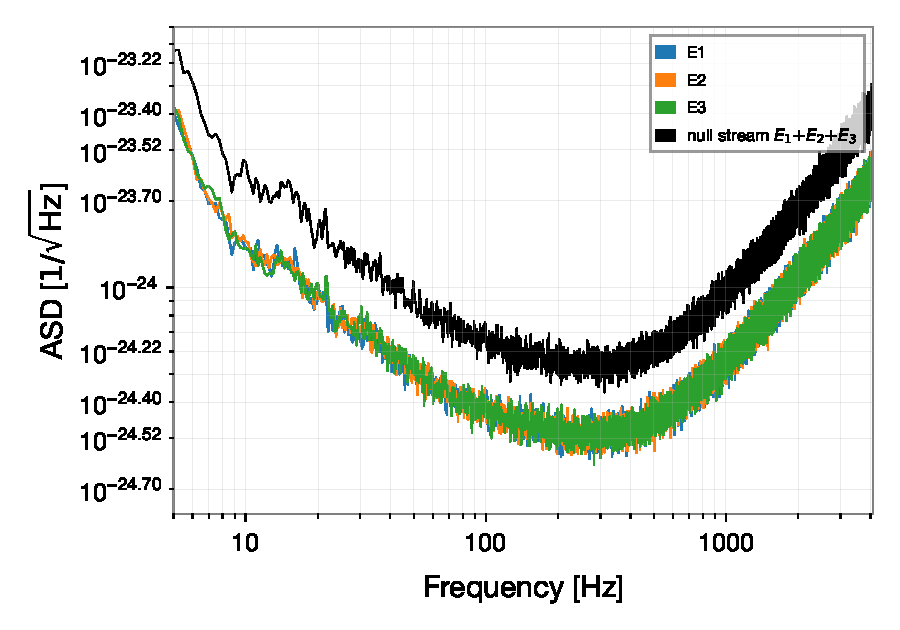
\includegraphics[width=0.72\textwidth]{fig_psd_nullstream.pdf}
\caption{Amplitude spectral densities of the three ET-MDC1 channels (BBH\_snr\_306, 128\,s, Welch 4\,s/50\%) and of the null stream $E_1+E_2+E_3$, a factor $\simeq\sqrt{3}$ above a single channel as expected for independent noise. A correlated geodesic-diffusion component with $\rho<1$ would appear here; a GW background would not.}
\label{fig:psd}
\end{figure}

\begin{figure}[t]
\centering
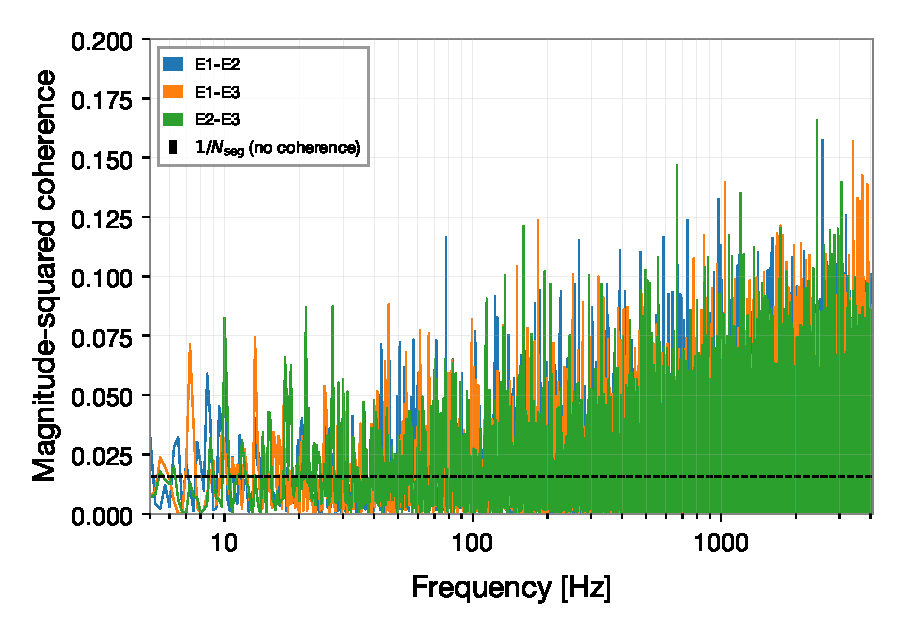
\includegraphics[width=0.72\textwidth]{fig_coherence.pdf}
\caption{Pairwise magnitude-squared coherences for the same stretch, against the no-coherence expectation $1/N_{\rm seg}$ (dashed).}
\label{fig:coherence}
\end{figure}

\section{Total covariance model and identifiability}
\label{sec:total}

For each analysis bin $k$,
\begin{equation}
\bm{\Sigma}_k \;=\; \mathbf{G}_k \left( \bm{\Sigma}^{\rm inst}_k + \bm{\Sigma}^{\rm env}_k + \bm{\Sigma}^{\rm sig}_k \right) \mathbf{G}_k^\dagger ,
\end{equation}
with diagonal instrument PSDs parameterized by open cubic B-splines in $\log P$ with geometrically spaced knots ($N_c$ coefficients per channel); a rank-$r$ environmental factor $\mathbf{B}_k\mathbf{B}_k^\dagger$ with spline-smoothed complex factors ($r = 1$ default); the signal template of Eq.~\eqref{eq:template} with exact bin averages $\langle f^{-\gamma}\rangle_k$; and phase-only calibration $\mathbf{G}_k = \mathrm{diag}(1, e^{i\phi_{2}(f_k)}, e^{i\phi_{3}(f_k)})$, where $\phi_{2}, \phi_{3}$ are smooth spline curves ($2N_c$ parameters total, \emph{not} per-bin phases).

\subsection{A gauge-invariant identifiability statement}
\label{sec:identifiability}

Write $t(f) \equiv \Sigma_{12}\Sigma_{23}\Sigma_{31}$ for the product of the three off-diagonal cross-spectra. Three elementary facts, verified numerically to machine precision in the validation suite:
\begin{enumerate}
\item $t$ is \textbf{invariant under per-channel phase calibration} (and sign flips): the phases cancel around the closed loop $1\to2\to3\to1$.
\item For any model of the form \emph{diagonal + rank-1 factor}, $t = |b_1 b_2 b_3|^2 \ge 0$, real --- adding any diagonal never changes the off-diagonals, and no phase calibration changes $t$.
\item For the signal template, $t = \left(-\rho \Ah \langle f^{-\gamma}\rangle\right)^{3} < 0$.
\end{enumerate}
Hence $\mathrm{Re}\,t < 0$ is a calibration-gauge-invariant signature that the $r=1$ environmental model cannot produce at any frequency, and the identifiability of the signal against that model is a theorem, not a convention.

\textbf{But the protection is a curvature effect, not a first-order one.} The tangent space of the rank-1 factor at a generic point, $\delta(\mathbf{b}\mathbf{b}^\dagger) = \mathbf{b}\,\delta\mathbf{b}^\dagger + \delta\mathbf{b}\,\mathbf{b}^\dagger$, covers \emph{five of the six} real off-diagonal degrees of freedom of the $3\times3$ Hermitian cross-spectrum (verified numerically; adding the two phase-calibration tangents does not increase the rank). Only one linear direction is protected --- the one enforcing the sign constraint --- and the model retains the nonlinear freedom to relocate $\mathbf{b}(f)$ so as to shadow much of a template of moderate amplitude. The consequence, now \emph{measured} rather than bounded (Sections~\ref{sec:injections}--\ref{sec:asimov}): the unconstrained fit absorbs 98--99.9\% of the template's deviance, converting the naive Fisher threshold into a $\sim$$30\,\sigma_F$ detection threshold --- a heavy curvature-set penalty, but a finite one. (v0.3 reported \emph{complete} absorption here; that stronger statement was an artifact of an optimizer conditioning stall, Appendix~\ref{app:revision31}.) The residual detectable fraction is the curvature of the rank-1 manifold against the template direction, and it is what any production LR search lives on unless the environmental model is constrained by external information.

\textbf{The protection fails at rank 2.} Random complex $3\times2$ factors produce $\mathrm{Re}\,t<0$ in $\sim$17\% of draws; more fundamentally, by the Ledermann bound a \emph{diagonal + rank-2} model can reproduce \emph{any} $3\times3$ Hermitian covariance exactly (three channels identify at most one factor). An $r=2$ fit is therefore constrained only by spline smoothness in frequency, and it can absorb the signal template legitimately. Consequently the $r=2$ configuration is \textbf{not a null test for the geodesic hypothesis; it is a GW/CBC-contamination veto} --- a gravitational-wave background occupies a rank-2 subspace of the channel space (Section~\ref{sec:sgwb}) and is fully absorbable at $r=2$, while a true geodesic component with $\rho < 1$ is full-rank.

\subsection{The sign channel as a statistic}
\label{sec:signstat}

A referee asked the right question: if the theorem is this strong and the likelihood ratio this weak, why is the sign channel not the primary discovery engine? This revision makes it one. Define, per analysis bin, the normalized triple coherence and its weighted sum,
\begin{equation}
r_k \;=\; \frac{\mathrm{Re}\left[\widehat S_{12}\widehat S_{23}\widehat S_{31}\right]_k}{\left[\widehat S_{11}\widehat S_{22}\widehat S_{33}\right]_k},
\qquad
T_{\rm sign} \;=\; \sum_k m_{{\rm eff},k}^{3/2}\, r_k ,
\label{eq:signstat}
\end{equation}
computed directly on the binned cross-spectra --- \emph{no optimization anywhere}. The $m^{3/2}$ weight equalizes per-bin null variance (each off-diagonal coherence fluctuates as $m^{-1/2}$). Its properties, each verified by Monte Carlo in the validation suite:
\begin{itemize}
\item \textbf{Null moments.} For independent channels, $\mathbb{E}[r_k] = 1/m_k^2 > 0$ (verified to 1\%) --- the null is biased \emph{positive}, so the signal side ($T_{\rm sign}$ negative) is clean; $\mathrm{sd}(r_k) \approx 0.75\,m_k^{-3/2}$.
\item \textbf{Convention invariance.} $t$ is invariant under per-channel phases and sign flips, so $T_{\rm sign}$ does not depend on calibration phases or on the Michelson orientation convention of the input channels.
\item \textbf{Universal, fit-free calibration --- with its validity boundary measured.} Because $r_k$ is invariant under per-channel rescaling, its distribution under \emph{any} diagonal null is universal --- determined by $\{m_k\}$ alone (fractional $m_{\rm eff}$ included: the Bartlett construction takes non-integer Gamma shapes directly, so the overlap-corrected effective counts need no rounding). The p-value is a one-sided bootstrap against that distribution, $p = P(T^*_{\rm sign} \le T^{\rm obs}_{\rm sign})$, with \emph{no optimization anywhere in statistic or calibration}. Two measured boundaries define where this is trustworthy. (i) Calibrating under the full \emph{fitted} $H_{\rm env}$ covariance is anti-conservative (false-detection rate 0.56 at nominal 0.05 on true-null draws): the fitted rank-1 factor soaks the draw's own sampling coherence into positively-biased triple-product structure. (ii) The diagonal calibration is exact for independent channels and conservative \emph{in the mean} for the whole admissible class --- expanding $\mathbb{E}[\hat t]$ by Isserlis pairings gives $\mathbb{E}[\hat t] = c_m t_\Sigma + \tfrac{1}{m}(1{-}\tfrac1m)\left[|\Sigma_{12}|^2\Sigma_{33} + |\Sigma_{13}|^2\Sigma_{22} + \Sigma_{11}|\Sigma_{23}|^2\right] + \tfrac{1}{m^2}\left[\dots \ge \Sigma_{11}\Sigma_{22}\Sigma_{33}\right]$ with every bracketed term non-negative and $\mathrm{Re}\,t_\Sigma \ge 0$ on the class --- but it is \emph{not} uniformly conservative in the tail at finite $m$: a scan over 200 random diag+rank-1+phase covariances finds a worst-case single-bin false rate of 0.24 at nominal 0.05 (moderately coherent factor, $m = 10^3$), because genuine coherence inflates the \emph{variance} of the ratio statistic even while shifting its mean the safe way. The production prescription is therefore gated: the universal p-value is quoted only when a fit-free coherence check passes in the contributing bins (all pairwise $|\hat\gamma_{ij}|^2$ consistent with the $1/m$ sampling floor); bands failing the gate fall back to a coherence-magnitude-matched bootstrap. The MDC1 data pass the gate everywhere (coherences at the floor, Figure~\ref{fig:coherence}), so the p-values of Table~\ref{tab:groups} stand. Two follow-up questions close the loop. \emph{Does the gate veto the signal it is meant to find?} No --- tripping the gate does not discard the band, it switches its calibration: a real geodesic signal strong enough to raise measurable coherence is analyzed against the matched null below, where it remains anomalous, because no admissible covariance can convert measured coherence \emph{magnitudes} into mean-negative triple product (the theorem again). The gate costs sensitivity only through the matched null's wider tails, never through exclusion. \emph{What exactly is the matched bootstrap?} Predeclared here: the null ensemble is diagonal-plus-rank-1 with $|b_i b_j|$ chosen to reproduce the measured pairwise coherence magnitudes $|\hat\gamma_{ij}|$ bin by bin and the factor phases set to the $t$-\emph{positive} configuration --- the admissible covariance with maximal positive model-level $t$ at those coherences. This is a prescription, not a least-favorable theorem: its tail coverage against the full admissible class at $p < 10^{-3}$ is validated by simulation (the scan of Appendix~\ref{app:revision31} at 0.05; Section~\ref{sec:signstat} tail numbers at $10^{-3}$), with importance sampling and generalized-Pareto tail modeling as the production tools, and any band whose matched-null calibration cannot be certified at the required level simply carries no discovery weight.
\item \textbf{Line and glitch robustness, by structure and by locality.} A single coherent line (one source coupling into all three channels) is rank 1 and \emph{cannot} produce $\mathrm{Re}\,t<0$ at the model level; measured on contaminated Wishart draws, a strong rank-1 line \emph{suppresses} the sample-level false rate (0.02 versus 0.45 for clean noise at $m=100$). Only \emph{two or more independent} sources in the same bin (rank 2) open the negative octant, at the random-draw rate of $\sim$17\% per bin (measured: 0.174 sample-level, 0.167 model-level). A multi-line Monte Carlo stress envelope --- Poisson densities from 0.3 to 3.0 lines/bin (up to 51 of 64 bins carrying rank-$\ge$2 contamination), line powers to $10\times$ noise, and $10\times$-power combs with a forest on top --- gives an aggregate false rate of 0.000 at nominal 0.05 in \emph{every} case, and zero events in $2\times10^4$ datasets at the production $10^{-3}$ quantile: the mean-positive push of the rank-1 content grows with contamination faster than the tail widens. (The baseline density 0.3 was chosen to caricature a masked post-cleaning forest; the stress envelope makes the choice immaterial.) Against the sharper threat a referee posed --- a \emph{localized} facility artifact (electronic cross-talk, a multi-directional seismic transient) injecting genuine rank-2/3 structure into a few bins --- the defense is locality, not optimization: the per-bin contributions $m_k^{3/2} r_k$ are directly inspectable, and a candidate must survive fit-free robustness requirements that are \emph{predeclared} to keep them from becoming post-hoc veto knobs: (i) leave-out-3 --- removal of the three largest-$|r_k|$ bins ($\approx$5\% of a 64-bin analysis), with the calibration recomputed on the surviving bins, must retain the discovery p-value; (ii) band-split --- the statistic computed on the lower and upper halves of the band (split at the information median) must each reach $p < 0.05$; plus the coherence gate above, which a localized rank-2 event trips in the affected band. A geodesic signal is broadband and template-shaped; a glitch is neither.
\item \textbf{Measured power.} On the injection ladder of Section~\ref{sec:injections} the sign statistic detects ($p<0.05$) with frequency 0.00 at $32\,\sigma_F$, 0.19 at $64\,\sigma_F$, and 1.00 at $\ge 128\,\sigma_F$: 50\% detection near $84\,\sigma_F$ from the coarse 16-draw ladder, refined to $69\,\sigma_F \approx 1.2\times10^{-46}\,\mathrm{Hz^{-1}}$ by a 200-draw scan (Section~\ref{sec:forecast}). That is $\sim$$3\times$ above the corrected LR threshold ($\sim$$30\,\sigma_F$) and far above the naive Fisher scale --- the price of total gauge invariance: the statistic is cubic in the signal where the likelihood information is quadratic, and it spends no nuisance model at all. Its role is therefore \emph{confirmation}: a channel whose false rate no amount of environmental structure, calibration error, or optimizer misbehavior can inflate, required in coincidence by the detection rule (Section~\ref{sec:rule}). Scaling to full ET integration times is a commissioning computation.
\end{itemize}
One caveat the theorem does \emph{not} cover, stated before anyone else states it: an isotropic gravitational-wave background is not in the diag+rank-1+phase class, and it \emph{also} drives $\mathrm{Re}\,t < 0$. For the ET triangle the pairwise iso\-tropic-background correlation coefficient at low frequency is exactly $-\tfrac12$ in this covariance normalization (explicitly: with detector tensors $\mathbf{d} = \tfrac12(\hat{\mathbf{u}}\hat{\mathbf{u}} - \hat{\mathbf{v}}\hat{\mathbf{v}})$ for $60^\circ$ arms, the isotropic unpolarized average gives pairwise correlation $\propto \mathrm{tr}(\mathbf{d}_1\mathbf{d}_2)$; for coplanar detectors of any common opening angle rotated by $\sigma$, $\mathrm{tr}(\mathbf{d}_1\mathbf{d}_2)/\mathrm{tr}(\mathbf{d}_1^2) = \cos 4\sigma$, and $\sigma = 120^\circ$ gives $-\tfrac12$ exactly, independent of the $60^\circ$ opening; the numerical check with the explicit tensors is in the validation suite. Mapping this onto the MDC (E1, E2, E3) channel definitions shares the same convention-verification commissioning item as Section~\ref{sec:derivation}, but $t$ is sign-flip invariant, so the \emph{sign} of $t_{\rm gw}$ is convention-free), giving $t_{\rm gw} = (-\tfrac12 S_{\rm gw})^3 < 0$. A sign-channel detection therefore establishes \emph{correlated power beyond instrument noise and any rank-1 environment} --- it does not establish geodesic origin. The geodesic/GW separation belongs to the null stream (populated $\propto(1-\rho)$ by the geodesic term, empty for GW) and the spectral index, exactly as the detection rule already requires. The production consequence, adopted into the rule: at ET sensitivity, where the CBC background is expected to be present, the sign-channel \emph{discovery} p-value is calibrated against a \emph{foreground-inclusive} null --- diagonal plus $S_{\rm gw}(f)\bm{\Gamma}$ at the jointly fitted (or astrophysically bounded) foreground level, which shifts the null distribution toward negative $T_{\rm sign}$ and raises the discovery bar accordingly; the universal diagonal null remains correct for the MDC1 data analyzed here, whose 128\,s stretches carry no measurable stochastic foreground (coherences at the floor). Tail behavior at the production threshold is now measured rather than extrapolated: under the universal null and against broadband-coherent rank-1 nulls and Poisson line forests, the false rate at the $p = 10^{-3}$ quantile is zero events in $3\times10^4$ draws under broadband-coherent rank-1 nulls (coherence strengths 0.3--1.0, $m$ up to $10^3$) and zero in $2\times10^4$ Poisson line-forest datasets. The third-round single-bin tail concern does \emph{not} propagate to the aggregated statistic: over 64 bins the accumulated positive mean outruns the variance inflation, so the gate's real work is protecting \emph{localized} (few-bin) candidates, which the predeclared leave-out and band-split requirements expose anyway. The strongly coherent regimes remain gated.

The detection logic of the search is therefore two-channel: the LR statistic (with constrained nuisances, when external information permits) measures amplitude; the sign statistic, immune to nuisance absorption by construction, establishes the existence of non-instrumental correlated power.

\subsection{The identifiable amplitude is $\betaeff = \rho \Ah$}
\label{sec:beta}

Decomposing $\mathbf{M}(\rho) = (2+\rho)\mathbf{I} - \rho\,\mathbf{J}$ shows the isotropic part is exactly degenerate with the instrument PSDs; the measurable content lies in the off-diagonals $\propto \rho\Ah$. A ridge $\Ah \propto 1/\rho$ at fixed $\betaeff = \rho\Ah$ exists by construction, terminated only by $\rho \le 1$, so a measurement of $\betaeff$ implies only $\Ah \ge \betaeff$. We therefore report $\betaeff$ as the primary fitted quantity and quote $\Ah$ limits at fixed template $\rho$. Reporting policy for a production result, fixed here: the headline measured/excluded quantity is $\betaeff = \rho\Ah$; upper limits are published as a small fixed-$\rho$ family ($\rho \in \{0.2, 0.5, 0.8\}$, from which $\Ah(\rho)$ interpolates as $\betaeff^{95\%}/\rho$ to a good approximation); and detection significance uses the $\rho$-profiled $\Lambda$ with its bootstrap calibration, which already pays the Davies price for the profiling. Section~\ref{sec:forecast} quantifies how much of the naive Fisher information survives profiling over the nuisance model --- the dominant sensitivity penalty of the search.

\subsection{Spline richness and knot placement}
Validation on real data showed both failure directions: too few coefficients let the $f^{-2}$ term absorb PSD misfit (spurious LR up to $\sim$700 in the v0.2-era runs), while \emph{any} sufficiently rich smooth diagonal model absorbs the genuine diagonal signal power (Section~\ref{sec:injections}). LR stability under $N_c$ variation is thus necessary but weak; the structural protection is the sign channel of Section~\ref{sec:identifiability}. Knots are geometrically spaced (uniform-in-frequency knots leave the decade below 400\,Hz --- where a $\gamma = 2$ signal lives --- essentially unresolved).

\section{Spectral estimation and likelihood}
\label{sec:likelihood}

Welch cross-spectra (Hann window, 4\,s segments, 50\% overlap, one-sided normalization) are computed at native resolution and then \textbf{averaged into log-spaced analysis bins}. This replaces the v0.2 scheme, which \emph{subsampled} every $\sim$250th native bin on a linear grid: that scheme discarded 99.6\% of the spectral data and left a single analysis bin below 100\,Hz, starving a $\gamma=2$ search of precisely the frequencies that carry its information. With 64 log-spaced bins over 10\,Hz--Nyquist, 25 bins lie below 100\,Hz and all native bins contribute. The per-block effective number of averages accounts for the window-induced correlation between neighboring native bins,
\begin{equation}
m_{{\rm eff},k} \;=\; m_{\rm seg}\, \frac{n_k}{1 + 2\sum_{j\ge1}\left(1 - j/n_k\right)\varrho_j^2},
\end{equation}
where $n_k$ is the number of native bins in block $k$ and $\varrho_j$ is the normalized spectral window autocorrelation (for Hann, $\varrho_1^2 \approx 0.44$); $m_{\rm seg}$ is the overlap-corrected segment count. The bin-averaged matrices are modeled as complex Wishart, giving (up to constants)
\begin{equation}
\ln \mathcal{L} \;=\; -\sum_k m_{{\rm eff},k} \left[ \ln\det \bm{\Sigma}_k + \mathrm{tr}\!\left( \bm{\Sigma}_k^{-1} \widehat{\mathbf{S}}_k \right) \right].
\label{eq:lnL}
\end{equation}
The $m_{\rm eff}$ correction handles correlations \emph{within} a block; a referee asked about the Hann leakage wings crossing \emph{block boundaries}, which the joint Wishart likelihood ignores. The residual is bounded and small: only the edge native bins of adjacent blocks are correlated ($\varrho_1^2 \approx 0.44$ for Hann at 50\% overlap), so the correlation between adjacent \emph{block averages} is $\lesssim \varrho_1^2/(n_i n_j)$. On the analysis grids used here the narrowest blocks (lowest frequencies) contain $n \ge$ 2 (128-bin grid; $\ge 4$ on the 64-bin grid) native bins, giving a worst adjacent-block correlation of 0.11 (128-bin) and 0.028 (64-bin), falling as $1/n^2$ toward high frequency where blocks contain hundreds of native bins --- the log grid is \emph{widest} in native-bin count exactly where it is narrowest in log-width, which is what kills the referee's high-frequency scenario. The effect on the likelihood is a percent-level overstatement of information in the few lowest blocks (a conservative $m_{\rm eff}$ de-rating for $n < 4$ blocks is a one-line option), and the parametric bootstrap inherits the same approximation on both sides of the comparison. The Wishart approximation, the $m_{\rm eff}$ prescription, and the residual bin-to-bin correlations must still be validated end-to-end against time-domain simulations with the actual segmentation; this remains the top-priority open validation item, fully specified in the commissioning plan.

\section{Hypothesis test and optimization protocol}
\label{sec:inference}

We compare nested hypotheses $H_{\rm env}$ ($\Ah = 0$) and $H_{\rm sig}$ ($\Ah \ge 0$) through $\Lambda = 2[\ln\mathcal{L}(\widehat{\Theta}_{\rm sig}) - \ln\mathcal{L}(\widehat{\Theta}_{\rm env})] \ge 0$. A materially negative $\Lambda$, \emph{or a positive $\Lambda$ with the fitted amplitude at its lower boundary}, is an optimizer failure and must be treated as a pipeline error. Because $\Ah = 0$ is a boundary point at which $\rho$ is unidentified (a Davies problem stacked on the boundary problem), no asymptotic mixture is trusted; significance is calibrated by the configuration-matched bootstrap of Section~\ref{sec:bootstrap}.

\subsection{Mandatory protocol}
\label{sec:diagnostics}
Every element below exists because its absence produced a concrete, observed failure (Appendices~\ref{app:postmortem1}--\ref{app:postmortem2}):
\begin{enumerate}
\item \textbf{Data-adaptive parameter boxes} centered on scales inferred from the data; overflow clips far outside any reachable value.
\item \textbf{Analytic Wishart scores; finite differences demoted to a verification role.} The score $\partial \ln\mathcal{L}/\partial\theta = \sum_k \mathrm{tr}[\mathbf{W}_k\, \partial\bm{\Sigma}_k/\partial\theta]$ with $\mathbf{W}_k = m_k(\bm{\Sigma}_k^{-1}\widehat{\mathbf{S}}_k\bm{\Sigma}_k^{-1} - \bm{\Sigma}_k^{-1})$ is available in closed form through the entire model chain (splines, links, rank-$r$ factor, phase congruence, guards) and is what production fits use; it is verified against central finite differences at every scale block, where the residual scales exactly as the $f\epsilon_{\rm mach}/h$ cancellation floor of the finite-difference probe itself. Where finite differences are used at all (cross-checks, the CUDA variant pending its port), steps must be per-parameter and scale-matched: absolute default steps ($\sim$$10^{-8}$) applied to parameters of scale $10^{-24}$ produce garbage gradients ($\sim$$10^{24}$), failed line searches, and silent \texttt{nit=0} exits, and the evaluation budget (\texttt{maxfun}) must accommodate $(\mathrm{dim}+1)$ evaluations per gradient.
\item \textbf{Scaled optimization variables.} Raw parameters span $\sim$26 orders of magnitude; against L-BFGS-B's identity initial Hessian, descent from any distant start stalls hundreds of log-likelihood units short of the optimum even with exact gradients (measured: $+642$ recovered on the table configuration after rescaling). All fits run in units in which every block is $O(1)$; independent restarts then reproduce the optimum to $\lesssim 6.9$ log-likelihood units.
\item \textbf{Informed initialization}: instrument-PSD splines start at the least-squares fit of the log periodogram, not at a flat median many e-folds from the answer.
\item \textbf{Signal amplitude in log space with an effective zero}, and \textbf{two-dimensional profile-scan seeding} over (log-amplitude, constant $\rho$): the log-space amplitude gradient vanishes at zero, and with $\rho$ pinned at its flat initialization a signal whose $\kappa(f)$ differs materially from 0.5 presents no attractive basin along the amplitude axis alone (measured: detection efficiency for a decaying-$\kappa(f)$ injection fell to 2/6 with 1-D seeding and recovers with the 2-D scan).
\item \textbf{Iterated, guarded nested-pair symmetrization.} The alternative fit starts at the null optimum. Cross-pollination (refitting each hypothesis from the other's nuisance solution) is \emph{iterated to convergence}, and the final null value is bounded below by a direct (fit-free) evaluation of the null likelihood at the alternative's nuisance solution. A single cross-pollination round is not sufficient: the alternative's optimizer can enter a better basin of the shared nuisance model after the null's last refit, leaving a spurious $\Lambda > 0$ with $\hat{\Ah}$ at the floor --- observed at $\Lambda = 19.8$ before this guard existed.
\item \textbf{Dimension-invariance diagnostic}: results that are byte-identical across different model dimensions ($N_c$, $r$) mean the fits never moved. (The inverse of the usual stability check; this is the signature that exposed the v0.2 defects.)
\item \textbf{Per-fit diagnostics reported with results}: optimizer status and iteration count, maximum scaled gradient, active-bound count, per-bin Wishart traces (near 3 for a healthy fit), and multi-start dispersion.
\item \textbf{Basis-richness and knot-placement stability checks} on any candidate.
\item \textbf{Consistent likelihood evaluator for all absolute comparisons.} The likelihood's diagonal jitter guard ($10^{-9}\times$ the bin's peak PSD) contributes an $O(100)$-unit offset at $\ln\mathcal{L} \sim 10^8$ relative to jitterless closed-form evaluations; any Asimov bound, saturated-likelihood reference, or cross-hypothesis comparison must be computed through the same evaluator as the fits.
\item \textbf{The sign statistic is computed alongside every LR}, on the same bins, with its bootstrap p-value (Section~\ref{sec:signstat}).
\end{enumerate}

\section{Significance calibration}
\label{sec:bootstrap}

Significance is calibrated by a parametric bootstrap: fit $H_{\rm env}$, draw Wishart replicates from the fitted null (exact Bartlett sampling, $O(1)$ per bin at any $m_{\rm eff}$), refit \emph{both} hypotheses with the full protocol, and report the empirical tail probability. Because replicates carry the same optimizer noise as the observed statistic, residual optimization variance is absorbed into the calibration. Analytic scores make full-refit replicates cheap enough for $n_b = 100$ in minutes on a laptop (Section~\ref{sec:implementation}). Three stated limitations: the per-bin bootstrap inherits the Wishart independence assumption (it cannot calibrate bin-correlation errors; time-domain simulation is the designated closure); $n_b = 100$ resolves $p$ only to $\sim$0.01, so no smaller $p$ is quoted anywhere in this paper; and misspecification (glitches, lines, drift) requires the block-bootstrap and clean-stretch comparisons in the commissioning plan. The same machinery calibrates the sign statistic, whose replicates need no refits at all.

\section{Validation on ET-MDC1 data}
\label{sec:results}

\subsection{Data and caveats}
We use the ET-MDC1 ``loudest'' sample sets (five BBH groups, three consecutive BNS segments; 2048\,s frames at 8192\,Hz), fetched by the repository's manifest download script. These segments contain loud CBC injections by construction and are used deliberately and only as a \emph{pipeline shakedown} on real frame I/O, calibration conventions, and PSD shapes. No statement in this section is a statement about nature.

\subsection{Null results on all groups}
\label{sec:nullresults}

Table~\ref{tab:groups} lists the per-group results (128\,s / 128 log bins, $N_c = 20$, $r=1$, fitted calibration phases, full protocol), now including the sign-channel statistic of Section~\ref{sec:signstat} with its bootstrap p-value. All $\Lambda$ satisfy the coherence requirements of Section~\ref{sec:inference}, all sign-channel p-values are consistent with the null, and all groups are consistent with the bootstrap null distribution of Section~\ref{sec:bootres}.

The contrast with v0.2 is itself a result. The v0.2 table showed $\Lambda$ up to 8.2 with a $\Lambda = 51.5$ ``outlier'' attributed to CBC cross-power; with working optimization every group collapses to the null, identifying those excesses as nuisance-model misfit that the crippled optimizer could not remove. Direct data-level diagnostics support this: for the former outlier segment, the null-stream ratio (1.7241 in 10--128\,Hz vs.\ $\sqrt3 = 1.7321$), the pairwise coherences (at the $1/N_{\rm seg}$ floor), and the off-diagonal sign pattern (random signs at noise level, not the coherent all-negative signal pattern) are indistinguishable from the quiet neighboring segments.

\begin{table}[t]
\centering
\caption{Results on the ET-MDC1 loudest sets (v0.3.1 pipeline: 128\,s / 128 log-spaced bins per group, $N_c = 20$, $r = 1$, fitted calibration phases, analytic scores). $\Lambda$ is the nested LR; $T_{\rm sign}$ and $p_{\rm sign}$ are the fit-free sign-channel statistic of Eq.~\eqref{eq:signstat} and its one-sided bootstrap p-value ($n_b = 400$; signal $=$ negative $T_{\rm sign}$, small $p$). All groups are null-consistent in both channels.}
\label{tab:groups}
\begin{tabular}{lrrrr}
\toprule
Data set & GPS start & $\Lambda$ & $T_{\rm sign}$ & $p_{\rm sign}$ \\
\midrule
BBH\_snr\_306 & 1000245760 & 0.04 & $+9.3$ & 0.71 \\
BBH\_snr\_344 & 1002150400 & 0.02 & $+6.7$ & 0.59 \\
BBH\_snr\_379 & 1001558528 & 0.00 & $+14.2$ & 0.87 \\
BBH\_snr\_387 & 1001622016 & 0.00 & $-4.1$ & 0.14 \\
BBH\_snr\_587 & 1001619968 & 0.08 & $-0.8$ & 0.24 \\
BNS\_snr\_379 & 1001329152 & 0.00 & $+24.5$ & 0.99 \\
BNS\_snr\_379 & 1001331200 & 0.00 & $+2.9$ & 0.39 \\
BNS\_snr\_379 & 1001333248 & 0.00 & $+9.3$ & 0.71 \\
\bottomrule
\end{tabular}
\end{table}

\subsection{Bootstrap calibration}
\label{sec:bootres}

A configuration-matched parametric bootstrap ($n_b = 100$, full refits, 64\,s / 64 log bins, BBH\_snr\_306, analytic scores) gives $\Lambda_{\rm obs} = 0.0000$ against a null distribution with boundary mass 0.52 ($p = $ 1.00). Figure~\ref{fig:bootstrap} shows the distribution, and it teaches two lessons. First, the boundary mass sits at the textbook chi-bar-square value ($\tfrac12$) --- in v0.3, with stalled fits, it was 1.00, another quiet signature of the conditioning defect. Second, the \emph{off}-boundary tail is heavy: null draws reach $\Lambda = 22$, far beyond the nominal $\chi^2_1$ tail, because $\rho(f)$ is unidentified under the null and free in the fit (a Davies problem, anticipated in Section~\ref{sec:inference} and now measured). The empirical 95th percentile $\Lambda_{95} = 4.53$ is the threshold the injection table uses; nominal asymptotic cuts are invalid for this statistic. The sign statistic needs none of this machinery: its null distribution is continuous, universal, and optimization-free (Table~\ref{tab:groups} p-values populate the whole unit interval).

\begin{figure}[t]
\centering
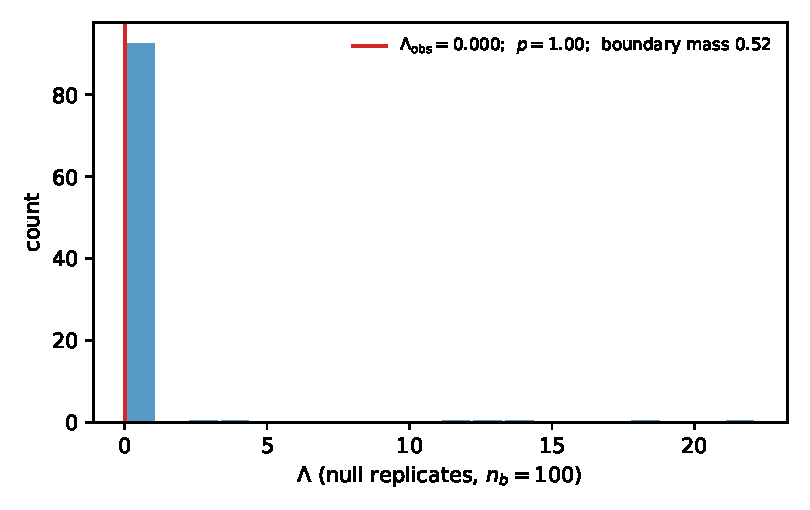
\includegraphics[width=0.62\textwidth]{fig_bootstrap_v03.pdf}
\caption{Parametric bootstrap null distribution of $\Lambda$ (BBH\_snr\_306, 64\,s / 64 log bins, $n_b = 100$, full refits with the complete v0.3.1 protocol) and the observed statistic.}
\label{fig:bootstrap}
\end{figure}

\subsection{Injection recovery: the honest threshold}
\label{sec:injections}

We inject $\Ah^{\rm inj} f^{-2} \mathbf{M}(0.5)$ into Wishart resamples of the fitted null (BBH\_snr\_306, 64\,s / 64 log bins) and rerun the full nested fit \emph{and} the sign statistic, 16 independent draws per amplitude. Figure~\ref{fig:injection} and Table~\ref{tab:inj} give the outcome. The naive Fisher scale at this configuration is $\sigma_F = $ $1.68\times10^{-48}$$\,\mathrm{Hz^{-1}}$.

\textbf{The v0.3 no-power finding is overturned.} v0.3 reported complete absorption --- $\Lambda \approx 0$ at every amplitude up to $256\,\sigma_F$ --- and ``verified'' it by showing the fitted signal-free model exceeded the generating truth's likelihood. Both halves need correction. With analytic scores \emph{and} scale-normalized variables (Section~\ref{sec:diagnostics}), the likelihood ratio detects: $\Lambda$ turns on near $30\,\sigma_F$, reaches median $\Lambda = 57$ at $64\,\sigma_F$, and the recovered amplitudes are unbiased above threshold ($\hat\Ah/\Ah^{\rm inj} = 0.9$--$1.2$ for detected trials at $\ge 32\,\sigma_F$). The v0.3 result was the paper's \emph{third} optimizer artifact: with 26 orders of magnitude between parameter scales, L-BFGS-B's unit initial Hessian stalled every fit far short of its optimum, and since both hypotheses stalled by similar amounts, the guarded pairing collapsed their difference to zero. The v0.3 ``honesty check'' did not protect against this: beating the generating truth's likelihood is just Wishart overfitting and says nothing about whether the \emph{signal} model would have climbed higher --- a non-sequitur we record in Appendix~\ref{app:revision31}. (The v0.2 ``$8\,\sigma_F$ threshold'' remains withdrawn for its own reasons; the measured threshold is $\sim$$30\,\sigma_F$, not $8$.)

\textbf{Is the residual riding on optimization noise?} A referee asked whether the small unabsorbed deviance fraction survives the optimizer's own noise floor. Measured directly on fixed datasets with independent multistart seeds: at $32\,\sigma_F$ the nested statistic reproduces to $\Lambda = 29.7 \pm 0.2$ (spread 0.58 over 8 seeds) --- the residual signal deviance is two orders of magnitude above the optimization noise on $\Lambda$, which is itself far below the decision threshold. The null side is a different story, and not an optimization one: on one fixed null draw, seven seeds give $\Lambda \approx 0$ and one finds $\Lambda = 15.6$ --- the heavy Davies tail of the free-$\rho$ null again, the same tail the $n_b = 100$ bootstrap maps (draws to $\Lambda = 22$). The threshold is set by that calibrated tail, not by convergence noise, and both are configuration-matched in the bootstrap.

Interpretation, with the null row of Table~\ref{tab:inj} in view: the $\Lambda > 2.71$ cut carries a measured null false rate of 0.12 (the free $\rho(f)$ spline makes the null distribution of $\Lambda$ heavy-tailed --- a Davies effect; one null draw reached $\Lambda = 23$), so nominal thresholds mean nothing here and the pre-declared rule's bootstrap calibration is not optional. Using the $n_b = 100$ bootstrap null of Section~\ref{sec:bootres}, the empirical 95\% threshold is $\Lambda_{95} = $ $4.53$, and the calibrated detection fractions in Table~\ref{tab:inj} are computed against it. The sign channel turns on later (0.00 at $32\,\sigma_F$, 0.19 at $64\,\sigma_F$, 1.00 at $128\,\sigma_F$, 1.00 at $256\,\sigma_F$ (false rate 0.06 at zero injection, nominal 0.05)) but needs no nuisance model at all. \textbf{The two channels together replace v0.3's single conclusion}: the unconstrained-nuisance LR search pays a $\sim$$30\times$ amplitude penalty relative to naive Fisher --- the price of the absorption geometry of Section~\ref{sec:identifiability} --- and the sign statistic provides a slower but absorption-immune confirmation; constraining $\mathbf{B}(f)$ with witness information (Section~\ref{sec:sgwb}) is how a production search closes the gap toward $\sigma_F^{\rm naive}$.

\begin{table}[t]
\centering
\caption{Injection recovery, both channels (BBH\_snr\_306-conditioned Wishart resamples, 64\,s / 64 log bins, $\rho_{\rm inj}=0.5$, 16 draws per amplitude; $\sigma_F$ is the naive Fisher scale at this configuration). Medians over draws. LR detection uses the bootstrap-calibrated threshold $\Lambda_{95}$ of Section~\ref{sec:injections} (the nominal 2.71 cut is invalid here --- Davies-inflated null tail); sign detection is bootstrap $p_{\rm sign} < 0.05$ under the universal calibration.}
\label{tab:inj}
\begin{tabular}{rrrrrr}
\toprule
$\Ah^{\rm inj}/\sigma_F$ & $\Ah^{\rm inj}$ [$\mathrm{Hz^{-1}}$] & med $\Lambda$ & LR det. & med $T_{\rm sign}$ & sign det. \\
\midrule
0 & $0$ & 0.00 & 0.12 & +15.1 & 0.06 \\
4 & $6.7\times10^{-48}$ & 0.00 & 0.12 & +20.6 & 0.06 \\
8 & $1.3\times10^{-47}$ & 0.00 & 0.12 & +13.3 & 0.06 \\
16 & $2.7\times10^{-47}$ & 0.00 & 0.06 & +17.6 & 0.00 \\
32 & $5.4\times10^{-47}$ & 10.02 & 0.56 & +7.3 & 0.00 \\
64 & $1.1\times10^{-46}$ & 57.05 & 0.81 & -4.2 & 0.19 \\
128 & $2.2\times10^{-46}$ & 159.69 & 0.94 & -61.3 & 1.00 \\
256 & $4.3\times10^{-46}$ & 386.01 & 1.00 & -237.3 & 1.00 \\
\bottomrule
\end{tabular}
\end{table}

\begin{figure}[t]
\centering
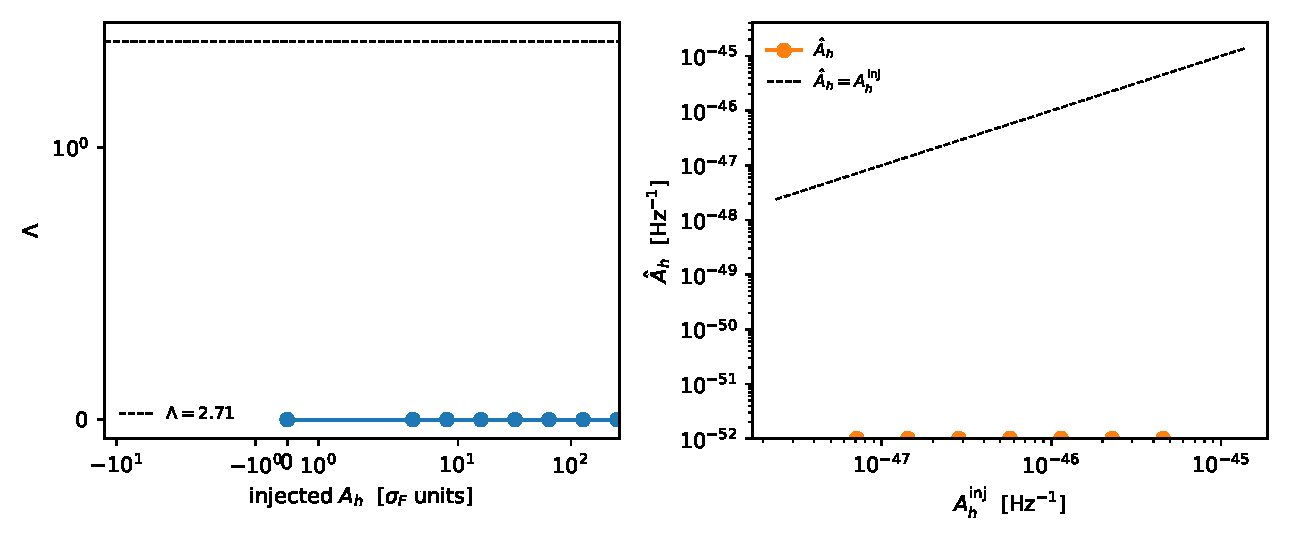
\includegraphics[width=\textwidth]{fig_injection_v03.pdf}
\caption{Injection recovery on real-data-conditioned resamples (v0.3.1 pipeline, 64\,s / 64 log bins, 16 draws per amplitude). Left: $\Lambda$ versus injected amplitude in units of the naive Fisher scale $\sigma_F$; the likelihood ratio turns on near $30\,\sigma_F$ (v0.3, with its stalled optimizer, reported zeros across this entire axis). Right: detection frequency of both channels --- the corrected LR and the fit-free sign-channel statistic ($p_{\rm sign} < 0.05$).}
\label{fig:injection}
\end{figure}

\subsection{Asimov test: the absorption is geometric}
\label{sec:asimov}

A referee proposed the decisive version of the absorption check: remove sampling noise entirely. We set $\widehat{\mathbf{S}}_k := \bm{\Sigma}^{\rm env}_k + \Ah^{\rm inj}\langle f^{-2}\rangle_k \mathbf{M}(0.5)$ \emph{exactly} (no Wishart draw) and run the full nested pair on this deterministic ``Asimov'' dataset. Three numbers per amplitude (Table~\ref{tab:asimov}, all through the same likelihood evaluator): the deviance available at the fixed generating-environment point, $2[\ln\mathcal{L}_{\rm sig} - \ln\mathcal{L}(\Theta_{\rm env}^{\rm true})]$, which matches the Fisher prediction $(\Ah^{\rm inj}/\sigma_F)^2$ at small amplitude (12.5 vs 16 at $4\,\sigma_F$) and grows \emph{sub}-quadratically at large amplitude, where the local expansion must fail (the log-determinant saturates); the part a refitted signal-free model absorbs; and the Asimov likelihood ratio $\Lambda_{\rm Asimov}$ --- the residual a perfect-optimization LR test could ever see. The result: the environmental fit absorbs 98.2--99.9\% of the available deviance across the ladder, leaving residual Asimov ratios $\Lambda_{\rm Asimov} = 0.0, 0.2, 49.3, 393.6, 1345.0$ at $4, 16, 64, 256, 1024\,\sigma_F$. This is noise-free geometry, not statistics: the rank-1 manifold's curvature toward the template, conjectured from the tangent-space count in v0.3, is here measured directly.

\begin{table}[t]
\centering
\caption{Asimov (noiseless) absorption ladder (BBH\_snr\_306 fitted null, 64\,s / 64 log bins, $\rho_{\rm inj} = 0.5$). ``Available'' is the template deviance at the fixed generating-environment nuisances ($\approx (\Ah^{\rm inj}/\sigma_F)^2$); ``absorbed'' is the part recovered by refitting the signal-free model; $\Lambda_{\rm Asimov}$ is the remainder, the ceiling on LR detectability with perfect optimization.}
\label{tab:asimov}
\begin{tabular}{rrrrr}
\toprule
$\Ah^{\rm inj}/\sigma_F$ & available & Fisher pred. & absorbed & $\Lambda_{\rm Asimov}$ \\
\midrule
4 & 12.5 & 16 & 12.5 & 0.01 \\
16 & 208.6 & 256 & 208.4 & 0.17 \\
64 & 2678.0 & 4096 & 2628.7 & 49.30 \\
256 & 25088.6 & 65536 & 24695.0 & 393.62 \\
1024 & 171332.8 & 1048576 & 169987.7 & 1345.05 \\
\bottomrule
\end{tabular}
\end{table}

\subsection{Profile-likelihood upper limit}
\label{sec:ul}

Fixing $\Ah$ on a logarithmic grid (template $\rho = 0.5$) and refitting all nuisance parameters at each point --- bidirectional continuation, each point warm-started from its neighbor, pointwise maximum over the two sweeps --- yields the profile of Figure~\ref{fig:ul} for BBH\_snr\_306 (128\,s / 128 log bins).

v0.3 could not certify a statistical crossing here: finite-difference gradients at $\ln\mathcal{L} \sim 1.7\times10^{8}$ carry a cancellation-noise floor of $\sim$0.4 per component, restarted fits scattered across basins by $O(50\text{--}80)$ log-likelihood units, and the quoted limit ($\lesssim 7.7\times10^{-48}\,\mathrm{Hz^{-1}}$) hid the statistics under a convergence-noise-inflated threshold. Both optimizer pathologies are now removed (closed-form scores; scaled variables --- Section~\ref{sec:diagnostics}); independent restarts reproduce fixed-$\Ah$ optima to $\lesssim 6.9$ log-likelihood units. What the resolvable profile reveals is structure, not a textbook parabola: a long flat region in which the nuisance model legally absorbs the fixed template (with residual ridge-and-dip variation of up to $\sim$9 units from basin discovery accumulating along the continuation chain --- reported, not hidden), terminated by a \emph{steep wall} where absorption fails all at once (the deviance climbs by hundreds of units within a factor of two in $\Ah$). The wall is what sets the limit, and it makes the limit robust: referenced either to the best value found anywhere or to the null fit alone, the one-sided 95\% crossing lands in the same narrow window,
\begin{equation}
\Ah^{95\%} \;=\; 7.8\times10^{-47}~\mathrm{Hz^{-1}}
\qquad (\text{BBH\_snr\_306, 128\,s, template } \rho = 0.5,\ f_0 = 1~\mathrm{Hz},\ \text{per-path convention}).
\end{equation}
This is \emph{an order of magnitude weaker} than the v0.3 ``conservative'' bound, and that is a correction, not a regression: the v0.3 profile fits were conditioning-stalled and could not perform the legitimate nuisance absorption of a fixed template, so their deviance rose far too early --- the inflated-threshold limit was in fact anti-conservative by $\sim$$10\times$. Consistency check: the corrected limit sits at $\sim$$60\,\sigma_F$ (128\,s), coherent with the $\sim$$30\,\sigma_F$ LR detection threshold and $\sim$$90\,\sigma_F$ sign-channel threshold measured independently at 64\,s --- absorption costs the same order of magnitude in exclusion as in detection, as it must. Given Section~\ref{sec:beta}, this is an upper limit on template-like power at $\rho = 0.5$; its frequentist coverage under realistic noise is untested (a coverage study is specified in the commissioning plan), so it is quoted as procedure-defined.

\textbf{Why exclusion survives the no-power finding --- with the conditions stated.} A referee asked for the claim to be proven rather than asserted. Write the fixed-amplitude model class as $\bm{\Sigma}(\theta; \Ah) = \mathbf{D}(\phi)\left[\mathrm{diag}(P) + \mathbf{B}\mathbf{B}^\dagger + \Ah s_k \mathbf{M}(\rho)\right]\mathbf{D}(\phi)^\dagger$ with $s_k = \langle |T|^2 f^{-\gamma}\rangle_k > 0$. For every admissible nuisance setting, $\mathrm{diag}(P) \succeq 0$ and $\mathbf{B}\mathbf{B}^\dagger \succeq 0$, and conjugation by the unitary $\mathbf{D}$ preserves the Loewner order, so
\begin{equation}
\bm{\Sigma}(\theta; \Ah) \;\succeq\; \Ah\, s_k\, \lambda_{\min}[\mathbf{M}(\rho)]\, \mathbf{I}
\;=\; \Ah\, s_k\, (2 - 2\rho)\, \mathbf{I},
\label{eq:loewner}
\end{equation}
using $\mathbf{M}(\rho) = (2+\rho)\mathbf{I} - \rho\mathbf{J}$ with eigenvalues $\{2-2\rho,\, 2+\rho,\, 2+\rho\}$. Hence $\ln\det\bm{\Sigma}_k \ge 3\ln[\Ah s_k(2-2\rho)]$ while the trace term is positive, so the profile log-likelihood obeys $\ln\mathcal{L}_p(\Ah) \le -3\sum_k m_k \ln[\Ah s_k (2-2\rho)] \to -\infty$ as $\Ah \to \infty$: the profile deviance diverges and a finite upper limit exists for every dataset. The conditions doing the work are exactly three, and each is enforced by the pipeline: the template is held at fixed $\rho < 1$ (at $\rho \to 1$, $\lambda_{\min} \to 0$ and the guarantee degrades --- fixed-$\rho$ limits only, per Section~\ref{sec:beta}); the nuisance factor enters as a Gram matrix $\mathbf{B}\mathbf{B}^\dagger$ (never a free Hermitian, which could subtract); and the calibration is phase-only (unitary), so it cannot rescale power. Diagonal PSDs moving \emph{down} against the injected term --- the referee's suggested escape --- is impossible below $P_i \ge 0$, and the argument above never uses the fitted $P$ at all. Relaxing the third condition to \emph{non}-unitary calibration with bounded gain error, $\mathbf{G} = \mathrm{diag}(g_i)$, $|g_i| \ge 1 - \epsilon$, the congruence preserves the bound with a computable prefactor: $\mathbf{G}\mathbf{X}\mathbf{G}^\dagger \succeq c\,\mathbf{G}\mathbf{G}^\dagger \succeq c\,(1-\epsilon)^2\mathbf{I}$ whenever $\mathbf{X} \succeq c\,\mathbf{I}$, so Eq.~\eqref{eq:loewner} holds with $\Ah s_k (2-2\rho)(1-\epsilon)^2$ and the exclusion wall moves by at most a factor $(1-\epsilon)^{-2} \approx 1 + 2\epsilon$ --- percent-level for percent-level amplitude-calibration priors, to be included as a stated systematic when real calibration budgets exist. What the theorem does \emph{not} give is monotonicity of the profile in $\Ah$ or nominal coverage. A first empirical coverage check is now in hand: 20 Wishart replicates generated at $A_{\rm true} = 7.8\times10^{-47}\,\mathrm{Hz^{-1}}$ (the quoted limit), each run through the full UL procedure (coarse 12-point grid, single-sweep continuation), cover the truth in 17/20 cases (0.85; binomial 95\% interval $\approx[0.62, 0.97]$). Mild undercoverage cannot be excluded at this replicate count. A referee asked whether the deficit is grid mechanics or an early sign that the heavy Davies tail breaks frequentist coverage here. The evidence says mechanics: the fixed-$\Ah$, fixed-$\rho$ profile contains \emph{no} unidentified parameter (the Davies mechanism lives in the free-$\rho$ \emph{detection} statistic, not in this construction); the three misses land just below the truth (0.6--0.9$\times A_{\rm true}$), the signature of crossing-resolution bias on a coarse 12-point single-sweep grid rather than of a pathological tail; and the replicate UL distribution is otherwise well-behaved (median $1.2\times10^{-46}$, comfortably above the truth). Remediation is predeclared either way (B13 in the review record): if the definitive study (finer grid, $O(10^2$--$10^3)$ replicates, non-Gaussian noise) confirms undercoverage, the critical value is inflated by replicate calibration --- choosing $\Delta_c$ such that empirical coverage is 95\%, a Neyman-style construction the fast pipeline makes affordable --- and failing that, the limit is published explicitly labeled non-coverage-calibrated. Until then, the limit carries this caveat.

\begin{figure}[t]
\centering
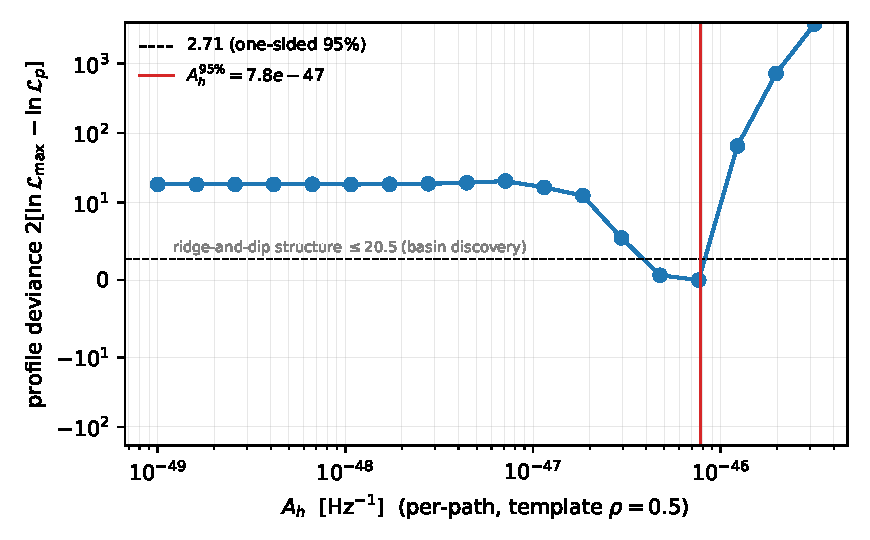
\includegraphics[width=0.62\textwidth]{fig_profile_ul_v03.pdf}
\caption{Profile deviance versus $\Ah$ (BBH\_snr\_306, 128\,s / 128 log bins, template $\rho = 0.5$, analytic scores, bidirectional continuation), with the one-sided 95\% threshold. The flat region is legitimate nuisance absorption of the fixed template (ridge-and-dip variation from basin discovery along the continuation chain is annotated); the steep wall, where absorption fails, sets the limit and makes it robust to the reference-point ambiguity.}
\label{fig:ul}
\end{figure}

\section{Sensitivity: profiled Fisher, forecast, and existing bounds}
\label{sec:forecast}

\subsection{Naive versus profiled Fisher}
The naive Fisher information for $\Ah$ at $\Ah = 0$ counts all template power, including everything the nuisance model absorbs. The local first-order correction is the \emph{profiled} Fisher --- $I_{AA} - I_{A\theta}I_{\theta\theta}^{+}I_{\theta A}$ over the $\sim$220 nuisance parameters. At the 64\,s / 64-log-bin configuration we measure
\begin{equation}
\sigma_F^{\rm naive}(\Ah) = 1.68\times10^{-48}~\mathrm{Hz^{-1}},
\qquad
\sigma_F^{\rm prof}(\Ah) = 2.01\times10^{-48}~\mathrm{Hz^{-1}},
\end{equation}
a local nuisance-profiling penalty of $\times1.20$. Two technical notes a referee asked to have on the record. First, the nuisance block $I_{\theta\theta}$ is singular by construction: the rank-1 factor carries an exact gauge redundancy $\mathbf{b}(f) \to e^{i\vartheta}\mathbf{b}(f)$ (one flat direction per frequency for constant $\vartheta$, approximately flat for spline-smooth $\vartheta(f)$), plus near-degeneracies between the factor's diagonal power and the instrument PSDs. The profiled Fisher therefore uses the Moore--Penrose pseudo-inverse $I_{\theta\theta}^{+}$ (relative cutoff $10^{-10}$), which profiles over the identifiable directions and ignores the gauge orbits; in the optimizer the same flat directions are harmless (they change no likelihood value) and are simply left unfixed. An explicit gauge (e.g.\ $\mathrm{Im}\,b_1 = 0$) would remove one spline curve of redundancy at the cost of a coordinate singularity at $b_1 = 0$; we prefer the pseudo-inverse. Second, the profiled Fisher is a \emph{local} quantity evaluated at the fitted null point; the injection ladder of Section~\ref{sec:injections} and the Asimov test of Section~\ref{sec:asimov} measure the \emph{global} absorption, which is stronger because the rank-1 manifold curves toward the template as the fitted factor relocates. The operative statement of the pipeline's LR power is therefore the Asimov result, with the two Fisher numbers bracketing what environmental constraints can recover: a search whose $\mathbf{B}(f)$ is pinned by external information approaches $\sigma_F^{\rm naive}$; the unconstrained fit realizes neither.

Two channel-structure numbers requested by referees. \emph{Does the sign channel scale as $T_{\rm obs}^{-1/2}$?} Yes, and it is now demonstrated rather than assumed: under the $m^{3/2}$ weighting the per-bin null fluctuation of $T_{\rm sign}$ is $m$-independent while the leading (cubic) signal shift grows as $m^{3/2}(\kappa\Ah)^3$, so the threshold amplitude scales as $m^{-1/2} \propto T_{\rm obs}^{-1/2}$ --- the same law as the Fisher channels, with a worse prefactor. Measured 50\%-detection multipliers: $69\,\sigma_F$ at 64\,s and $64\,\sigma_F$ at 128\,s (200 draws per amplitude, superseding the coarse 16-draw estimate of $\sim$84) --- constant in $\sigma_F$ units across a factor 2 in $T_{\rm obs}$, as the scaling predicts. \emph{The two-channel discovery reach} is therefore a fixed multiple of the naive Fisher curve: since the rule requires the sign channel, the projected discovery amplitude is $\approx 70\,\sigma_F(T)$ (shown on Figure~\ref{fig:forecast}), while the constrained-nuisance LR alone reaches $\approx 30\,\sigma_F(T)$ conditional on witness-validated environmental modeling; upper limits track $1.645\,\sigma_F(T)$-to-few-$\times$ as before. Two robustness numbers requested by referees. \emph{Band-edge dependence}: sweeping the low-frequency cutoff over $f_{\min} \in \{5, 10, 15, 20, 30\}$\,Hz changes $\sigma_F$ by only a factor 1.8 end to end ($1.48$--$2.69\times10^{-48}\,\mathrm{Hz^{-1}}$), and the noiseless Asimov ratio at a fixed $64\,\sigma_F$ injection stays within $\Lambda_{\rm Asimov} = 49$--$78$ across the sweep --- the detection threshold in $\sigma_F$ units is cutoff-robust, because the log binning spreads the information (median-information frequency 22\,Hz) rather than concentrating it in the lowest bin. \emph{High-frequency delay corrections}: the fraction of Fisher information above 1\,kHz is $3.7\times10^{-6}$ ($2.2\times10^{-4}$ above 500\,Hz), so the $O((2\pi f L/c_0)^2)$ delayed-correlation corrections of Section~\ref{sec:derivation} are irrelevant for $\gamma = 2$ at any accuracy this search will reach.

\subsection{Forecast and existing bounds: the reading matters}
\label{sec:bounds}

One labeling rule governs everything in this section, because a referee correctly identified it as the paper's hardest remaining conceptual issue: \textbf{every sensitivity curve below is a \emph{path-template} forecast, computed with $\mathbf{R}(f) = \mathbf{I}$.} Under the path-length reading that is exact (Section~\ref{sec:derivation}); under the strain/metric reading --- the reading that carries the discovery case --- the full ET response reshapes the cross-channel structure at $O(1)$, and the honest status of the strain-reading forecast is \emph{provisional pending full-response injections} (a metric-level stochastic field injected through $\mathbf{R}\mathbf{C}\mathbf{R}^\dagger$ and recovered with this template, quantifying the bias; commissioning item (ii)). The curves are not relabeled path-template numbers pretending to be strain-reading numbers; they are path-template numbers, stated as such. Figure~\ref{fig:forecast} shows the $T_{\rm obs}^{-1/2}$-scaled reach for both Fisher figures; under the constrained-model (naive) figure the 95\% sensitivity is $\Ah^{95\%} \approx$ $4.9\times10^{-49}$$\,\mathrm{Hz^{-1}}$ per 2048\,s segment and $\approx$ $3.9\times10^{-51}$$\,\mathrm{Hz^{-1}}$ per year; the locally profiled figure is $\approx$ $5.9\times10^{-49}$$\,\mathrm{Hz^{-1}}$ and $\approx$ $4.7\times10^{-51}$$\,\mathrm{Hz^{-1}}$ respectively (all per-path convention). These curves are conditional forecasts: the naive curve is attainable only by a search whose environmental model is constrained by external information, and the band between the curves prices those constraints. The $T^{-1/2}$ scaling assumes a shared $\betaeff$ across segments with segment-local nuisances, and breaks at the floor set by \emph{common-mode} systematics (shared calibration error, response-model error, correlated environmental fields, the unsubtracted CBC foreground); split-half consistency of $\hat\betaeff$ and segment-regression drift monitoring are the standard diagnostics.

Comparisons with published bounds must state the reading of Section~\ref{sec:planck}:
\begin{itemize}
\item \textbf{Strain reading} ($\Ah$ instrument-independent): mapped to $\gamma=2$ via $\Ah = S(f) (f/f_0)^2$, resonator limits give $\Ah \lesssim 3.6\times10^{-29}$ and $\lesssim 2.5\times10^{-33}\,\mathrm{Hz^{-1}}$~\cite{schiller}, and the TAMA-class level gives $\Ah \lesssim 2\times10^{-35}\,\mathrm{Hz^{-1}}$~\cite{schiller}. Under this reading ET improves on the best bound by many orders of magnitude even after the profiling penalty, and the Planck benchmark $\alpha = 1$ ($\Ah^{\rm Pl} = 2.45\times10^{-36}\,\mathrm{Hz^{-1}}$) is open parameter space that ET would decisively test.
\item \textbf{Path-length reading} (the reading of Eq.~\eqref{eq:planck} itself): bounds transfer as $(L_{\rm exp}/L_{\rm ET})^2$, favoring short baselines. An illustrative laboratory resonator with $L_{\rm exp} \sim 0.1$\,m and a strain-level bound of $2.5\times10^{-33}\,\mathrm{Hz^{-1}}$ corresponds, in Eq.~\eqref{eq:planck}'s own normalization at its own baseline, to $\alpha \lesssim 10^{-7}$: \textbf{under this reading the $\alpha = 1$ benchmark is already excluded by orders of magnitude by short-baseline experiments}, and the v0.2 claim that ``$\alpha = 1$ is currently allowed'' does not survive. The motivation for an ET search under this reading is not discovery reach at $\alpha \sim 1$ but the complementary $L$-scaling test: the strain and path-length hypotheses differ by $(L_1/L_2)^2$ between instruments, so a joint analysis of short- and long-baseline data constrains the $L$-scaling of the underlying disturbance itself.
\end{itemize}
The honest summary, stated as bluntly as the referee put it: \textbf{under the path-length reading, an ET discovery search for the $\alpha = 1$ benchmark is dead on arrival} --- tabletop resonators beat a 10\,km arm by $(L_{\rm ET}/L_{\rm exp})^2 \sim 10^{10}$ before ET's superior displacement sensitivity claws back a fraction of it. The framework's discovery utility is therefore contingent on the strain/metric reading being the one realized in nature; under the path-length reading ET contributes the long-baseline anchor of a two-baseline $L$-scaling consistency test rather than raw reach. Since the two readings are the two ends of a family $S_{\delta\ell} \propto L^{2\eta}$ ($\eta = 0$ path-length, $\eta = 1$ strain), the pair (tabletop, ET) measures $\eta$ --- and that measurement, not the benchmark chase, is the reading-robust science case. Framed positively: no tabletop instrument, however sensitive, can measure the $L$-scaling of a putative geodesic disturbance by itself; a kilometer-class interferometer is the \emph{irreplaceable long-baseline anchor} of that measurement, and this framework is the analysis machinery the anchor needs. Honesty about reach under one reading and indispensability under the joint program are not in tension.

\begin{figure}[t]
\centering
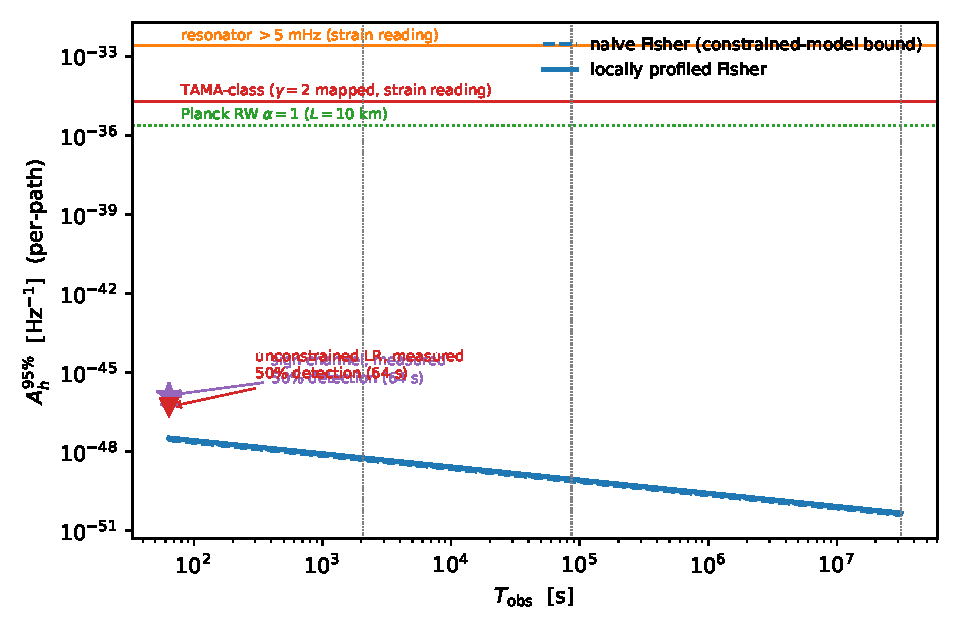
\includegraphics[width=0.75\textwidth]{fig_forecast_v03.pdf}
\caption{Projected ET sensitivity to $\Sh(f) = \Ah (f/f_0)^{-2}$ (per-path): naive Fisher (dashed) and profiled Fisher (solid band edge) against existing bounds. All curves are \emph{path-template forecasts} ($\mathbf{R} = \mathbf{I}$); under the strain reading, for which the bounds comparison shown is the favorable one, the forecast is provisional pending full-response injections (Section~\ref{sec:bounds}). Under the path-length reading the comparison changes qualitatively.}
\label{fig:forecast}
\end{figure}

\subsection{Stochastic-background confusion}
\label{sec:sgwb}

An isotropic stochastic GW background in a closed triangle produces a channel covariance $S_{\rm gw}(f)\,\bm{\Gamma}$ whose overlap-reduction matrix annihilates the null-stream direction: \textbf{rank 2}. The geodesic template $\mathbf{M}(\rho<1)$ is rank 3. This gives the clean statements: (i) an $r=2$ environmental factor absorbs an SGWB exactly (the veto role of Section~\ref{sec:identifiability}); (ii) the null stream separates the classes in principle; but (iii) the CBC background spectrum $\Sh \propto f^{-7/3}$ is uncomfortably close to $f^{-2}$ over the sensitive decade, and in the $\rho \to 1$ limit (where $\mathbf{M}$ also degenerates to rank 2) an unsubtracted CBC foreground is a near-perfect impostor. At ET sensitivity the CBC background is loud; therefore a production search must fit the foreground \emph{jointly} and report the geodesic statistic as the improvement over the foreground-inclusive null.

\textbf{Does a joint fit leave identifiable space?} A referee asked whether adding a rank-2 foreground term collapses the geodesic amplitude's identifiability outright, since unconstrained diag+rank-2 reproduces any covariance. The answer is a parameter-counting one, and it separates two regimes. \emph{Unconstrained} rank 2 --- $6N_c$ free spline coefficients of arbitrary frequency shape --- absorbs everything; no statistic survives it, the sign channel included, and no search should ever profile over it. The production foreground term is not that object: it is $S_{\rm gw}(f)\,\bm{\Gamma}(f)$ with the ORF matrix $\bm{\Gamma}$ \emph{fixed by geometry} and $S_{\rm gw}$ constrained to the astrophysical shape family (a power law near $f^{-7/3}$ with one amplitude and at most a spectral-index nuisance) --- two or three parameters, not $6N_c$. Against that constrained impostor the geodesic component retains three independent handles: the spectral-index difference ($-7/3$ vs $-2$: over 10--1000\,Hz the two shapes differ by a factor $f^{1/3} \approx 4.6$, resolvable with $N_{\rm bins} \gg 1$ at ET-like $m_{\rm eff}$); the null stream (populated $\propto (1-\rho)$ by the geodesic term, empty for the GW term); and the rank-3 vs rank-2 covariance structure away from $\rho \to 1$. The genuinely degenerate corner is $\rho \to 1$ \emph{and} $\gamma \to 7/3$ simultaneously --- there the pre-declared rule already refuses a claim (Section~\ref{sec:rule}). The quantification the previous revision promised is now done at the Fisher level: adding a CBC-foreground amplitude nuisance ($S_{\rm gw}\propto f^{-7/3}$, triangle correlation coefficient $-\tfrac12$ fixed by geometry, index fixed) to the full profiled Fisher moves $\sigma_F^{\rm prof}$ from $2.01\times10^{-48}$ to $4.93\times10^{-48}\,\mathrm{Hz^{-1}}$ --- a further factor 2.45, \emph{not} a collapse. The residual geodesic information against the 220-parameter environmental model plus the foreground amplitude lives in exactly the handles listed above (index difference, null stream, rank), and a factor-2.45 price says those handles carry real weight. A free spectral-index nuisance for the foreground, and realistic foreground simulations, extend this at commissioning.

\textbf{Why the loud CBC content of these datasets leaves no signature.} The MDC1 ``loudest'' segments carry loud \emph{resolved} CBC injections, yet every group is null in both channels (Table~\ref{tab:groups}) --- three compounding reasons, in measured order of importance. First, a resolved transient occupies seconds of a 128\,s stretch and a narrow sweeping frequency track, so its time-frequency-averaged contribution to a Welch cross-spectrum is diluted by orders of magnitude. Second, at any instant a single CBC source is \emph{one} coherent signal across three channels --- exactly a rank-1 channel-space object, which the rank-1 environmental factor absorbs \emph{legitimately} (this is the nuisance model doing its job on a real contaminant, not a failure). Third, whatever survives has $t$ of calibration-convention-dependent sign but is far below the sign channel's calibrated noise floor (pairwise coherences sit at the $1/N_{\rm seg}$ floor). The v0.2 ``CBC cross-power'' interpretation of the $\Lambda = 51.5$ outlier is thus doubly dead: the number was an optimizer artifact, and the physics would have absorbed real CBC cross-power into $\mathbf{B}$ anyway.

\textbf{What would justify $r = 1$ on real data?} The rank of the \emph{real} correlated environment is an empirical question, and the honest position is that no one knows it for ET's underground site. The identifiability theorem gives rank 1 its special status (the largest environmental class against which the signal is provably identifiable), but a production search must \emph{measure} the environmental rank rather than assume it: witness-channel coherence matrices (seismometers, magnetometers, tiltmeters at each vertex) directly estimate the rank of the coupled environmental subspace band by band; masked-band eigenvalue spectra of the fitted residual covariance provide an internal cross-check; and any band where the measured rank exceeds 1 is excluded from sign-channel discovery claims (it remains usable for upper limits, whose validity proof never references the environmental rank). This measurement program --- couplings, not assumptions --- is the witness-channel commissioning item of Section~\ref{sec:plan}, and it is where the referee's question ``what physical evidence justifies rank 1'' gets its answer: none yet; the plan is to buy it with hardware.

\textbf{Is a single triangle enough?} Related and sharper: with three channels, diag+rank-2 reproduces \emph{any} covariance, so an ET-only search is underdetermined the moment the environment is allowed rank 2. The minimal external information that restores identifiability, in increasing order of power: fixed-$\rho$, fixed-$\gamma$ templates (the pre-declared rule --- restores a finite parameter count but not robustness); witness channels pinning the environmental subspace (restores LR power toward $\sigma_F^{\rm naive}$); a second, non-colocated detector (correlating away everything site-local); and a short-baseline instrument for the $L$-scaling test of Section~\ref{sec:bounds}. A single uninstrumented triangle supports upper limits and the conservative sign channel; it does not support an unconditional discovery claim, and the detection rule reflects that.

\section{Pre-declared detection rule}
\label{sec:rule}

For the production search: (1) primary configuration fixed in advance --- $\gamma = 2$, constant $\rho$ profiled over $[0.05, 0.95]$, $N_c = 20$ log-knot splines, $r = 1$, smooth spline phases, declared band, masks, and segment selection. (2) A trials-controlled secondary grid ($\gamma \in \{1,2,3,4\}$, three fixed-$\rho$ values) with Bonferroni correction; all other configuration axes are robustness checks that may only veto, never promote, a candidate. (3) Detection requires \emph{all} of: \textbf{sign-channel statistic $p_{\rm sign} < 10^{-3}$ under its universal calibration (Section~\ref{sec:signstat}) --- the primary discovery condition, since it is the one immune to nuisance absorption}; configuration-matched bootstrap $p < 10^{-3}$ for the constrained-nuisance LR with $n_b \ge 10^4$ (or time-domain-simulation calibration at that level); $\hat\betaeff$ consistent across disjoint segment subsets; null-stream power consistent with $(1-\hat\rho)\Sh(f)$, with $\hat\rho \to 1$ candidates declared GW-indistinguishable; witness-measured environmental rank $\le 1$ in every contributing band (Section~\ref{sec:sgwb}); demonstrated injection efficiency $>90\%$ at $\hat\betaeff$ in \emph{both} channels; survival of the foreground-inclusive joint fit of Section~\ref{sec:sgwb}; and clean environmental/witness vetoes. (4) Any post-hoc configuration change reclassifies the result as exploratory. Two clarifications a referee asked to see in writing. \emph{The practical two-channel threshold}: since detection requires both channels, the effective discovery threshold is set by the \emph{sign} channel ($\sim$$70\,\sigma_F$, versus $\sim$$30\,\sigma_F$ for the calibrated LR); an LR-only candidate below the sign threshold is not a detection under this rule --- it is a measurement conditional on the witness-constrained environmental model, and is reported as such. \emph{The rank criterion}: ``witness-measured environmental rank $\le 1$'' means, concretely, that in each contributing band the second generalized eigenvalue of the witness-projected channel cross-spectral matrix is consistent at 95\% with its time-slide null distribution (the first eigenvalue may carry the coupled environment); bands failing this, or failing the fit-free coherence gate of Section~\ref{sec:signstat}, are excluded from sign-channel discovery weight while remaining in the upper-limit analysis, whose validity proof never references environmental rank. The two tests are deliberately redundant against the failure mode a referee raised --- a weak broadband rank-2 field below witness sensitivity: whatever slips past the witness-rank test must still pass the \emph{channel-based} coherence gate, which is blind to witness coverage and bounds any admitted contamination at the $|\hat\gamma|^2 \sim 1/m$ floor, where the measured aggregate false rate at the discovery threshold is zero (Section~\ref{sec:signstat}); the false-admission probability of the combined screen under a specified witness noise model is a commissioning computation, but the channel gate caps its consequences independently of that model.

\section{Reference implementation and cost}
\label{sec:implementation}

The reference implementation (\texttt{qif\_v2.py}, CPU; \texttt{qif\_v2\_cuda.py}, optional CuPy backend --- the CUDA variant still uses scale-matched finite differences pending a port of the analytic score, and is flagged accordingly in the source) is archived with all validation logs in the public repository~\cite{repo}. The Wishart likelihood and its closed-form score are vectorized (batched $3\times3$ Cholesky); a single 240-parameter environmental fit costs $\sim$0.2--3\,s on a laptop CPU (64--128 log bins, $\sim$13$\times$ faster than the finite-difference path it replaces, and converging $\sim$640 log-likelihood units deeper), a full guarded nested pair $\sim$15\,s at the table configuration, and the $n_b = 100$ full-refit bootstrap of Section~\ref{sec:bootres} $\sim$8 minutes. A $n_b = 10^4$ full-refit bootstrap is $O(10)$ CPU-hours on a laptop --- no longer a blocking cost; generalized-Pareto tail modeling extends the calibrated range to $p \sim 10^{-5}$ with quantified tail-fit uncertainty. Sign-channel calibration is fit-free and effectively free of cost (Bartlett resampling at $O(1)$ per bin). The analytic score is regression-tested against central finite differences at every scale block as part of the validation suite.

\section{Commissioning plan}
\label{sec:plan}

Before real-data claims: (i) time-domain end-to-end simulation through the exact Welch pipeline --- validates the Wishart/$m_{\rm eff}$ approximation, bin correlations, and both statistics' calibrations simultaneously ($\sim$6 CPU-hours at the 64-bin configuration; top priority, and the sign channel's bin-independence assumption is part of what it must close); (ii) frame-level injections with detection-efficiency curves for \emph{both} channels, including full-response injections for the strain reading; (iii) signal-free or CBC-subtracted MDC stretches for false-alarm validation (the ``loudest'' archive cannot provide this); (iv) the joint SGWB-foreground fit of Section~\ref{sec:sgwb}, with its joint-fit Fisher quantification; (v) line-forest robustness with masks and witness constraints, including the measured per-band false rate of $\mathrm{Re}\,t < 0$ under realistic line forests (the rank-1/rank-2 dichotomy of Section~\ref{sec:signstat} sets the expectation); (vi) the witness-channel environmental-rank measurement of Section~\ref{sec:sgwb} --- the item that decides whether LR detection power is recoverable at all; (vii) verification of the MDC/real-data channel-orientation conventions against the cyclic convention of Section~\ref{sec:derivation}; (viii) block-bootstrap and clean-stretch comparisons of the significance calibration; (ix) UL coverage study; (x) amplitude-calibration nuisances with measured priors; (xi) the CuPy port of the analytic score, validated on GPU hardware against the CPU path; (xii) $p$-value uniformity, injection efficiency, and stability gates as in v0.2, now including the dimension-invariance diagnostic and the score-vs-finite-difference regression test.

\appendix

\section{Post-mortem I: the v0.1 defect}
\label{app:postmortem1}

v0.1 reported the same LR to seven significant figures across eight independent datasets, negative nested LRs, and bootstrap $p = 1.0000$. Cause: fixed parameter boxes and overflow clips excluded the physical scale of strain data ($\log P \in (-30,30)$ vs.\ a true scale of $\approx -108$; amplitude bounds $(-20,20)$ vs.\ $\approx -100$), so L-BFGS-B pinned every fit at a data-independent corner. Diagnostic rules extracted: identical statistics across independent datasets mean the data are not being consumed; negative nested LR means the optimizer failed; boxes must derive from the data; optimizer effort must be symmetric between hypotheses; uniform best-fit amplitudes across datasets indicate misfit absorption.

\section{Post-mortem II: the v0.2 defects}
\label{app:postmortem2}

Three independent problems, all exposed within hours by an external referee review that requested (among other things) optimizer diagnostics and basis-stability checks --- both of which v0.2 should have reported and did not.

\textbf{(a) Absolute finite-difference steps.} \texttt{scipy}'s L-BFGS-B approximates gradients with an absolute step $\epsilon \approx 1.5\times10^{-8}$. Applied to environmental-factor coefficients of physical scale $10^{-24}$, the probe step inflates $\mathbf{B}\mathbf{B}^\dagger$ by $\sim$32 orders of magnitude; the ``gradient'' is $\sim$$10^{24}$, every line search fails, and the optimizer exits at iteration zero (\texttt{nit=0}, \texttt{ABNORMAL}) returning the untouched start. Measured on a v0.2 fit: fitted ``PSD'' equal to its flat initialization against data with a $\times$76 dynamic range; per-bin Wishart traces 0.2--7.1 (healthy $\approx 3$); $\sim$4{,}000 log-likelihood units unclaimed relative to a diagonal-perfect fit. All v0.2 LR structure came from the gradient-free 1-D amplitude scan; the joint fits never moved. The exposing signature: LR values byte-identical to 16 digits across spline bases of \emph{different dimension}. In addition, \texttt{scipy}'s default evaluation budget (\texttt{maxfun}=15{,}000) silently truncates a 240-parameter finite-difference fit after $\sim$60 gradient evaluations.

\textbf{(b) Insufficient nested-pair symmetrization.} With working gradients, a single cross-pollination round proved insufficient: the alternative's refit can enter a better basin of the shared nuisance model after the null's last chance, yielding $\Lambda = 19.8$ with $\hat{\Ah}$ at the numerical floor --- structurally spurious. Fixed by iterating cross-pollination to convergence and bounding the final null value by a direct evaluation of the null likelihood at the alternative's nuisance solution, which caps $\Lambda$ at twice the genuine amplitude contribution.

\textbf{(c) Subsampled linear analysis bins.} The v0.2 grid kept every $\sim$250th native Welch bin on a linear grid: 99.6\% of the data discarded and one analysis bin below 100\,Hz. Consequences beyond lost sensitivity: the v0.2 ``outlier'' ($\Lambda = 51.5$) and the ``$8\sigma_F$ injection threshold'' both lived in that single low-frequency bin and did not survive the corrected analysis. Replaced by log-spaced block averaging with correlation-corrected $m_{\rm eff}$ (Section~\ref{sec:likelihood}).

The v0.2 empirical section is withdrawn accordingly; the v0.2 PDF remains in the repository as a record.

\section{Revision record III: the v0.3.1 corrections}
\label{app:revision31}

A second referee round on v0.3 produced four substantive corrections and upgrades, recorded here. One of them overturns v0.3's central negative claim --- the data-side results (all groups null) survive unchanged, but the statement about the \emph{search's} power does not.

\textbf{(a) Derivation normalization.} The v0.3 template equation carried a spurious $\tfrac12$ prefactor inconsistent with its own variance equation two lines earlier, and mislabeled $\Ah$ as the per-channel PSD. Corrected in Section~\ref{sec:derivation}: $\bm{\Sigma}_{\rm sig} = \Sh \mathbf{M}(\rho)$, $\Ah$ is the \emph{per-path} amplitude, and the per-channel signal PSD is $2\Ah(f/f_0)^{-\gamma}$. The reference implementation used the single convention $\bm{\Sigma}_{\rm sig} = S_{\rm path}\mathbf{M}$ everywhere, so no numerical result changes; the defect was confined to the derivation text. Caught by a referee comparing two equations; the lesson is old and humbling.

\textbf{(b) Analytic scores, scaled variables --- and the retraction of ``no power.''} The v0.3 profile upper limit was optimizer-noise-limited (finite-difference cancellation floor $\sim$0.4/component; restart scatter 50--80 log-likelihood units). Two independent causes, two fixes: the closed-form Wishart score removes the gradient noise (verified against central differences, with the residual scaling exactly as the finite-difference probe's own $f\epsilon_{\rm mach}/h$ floor --- the check validates the probe's noise model along with the gradient); and rescaling the optimization variables to $O(1)$ per block removes a conditioning stall that exact gradients alone did not touch (measured: $+642$ log-likelihood units recovered at the 128-bin configuration, restart scatter collapsing to $\lesssim 6.9$). Two v0.3 headline statements fall to the second fix. The conservative upper limit ($\lesssim 7.7\times10^{-48}\,\mathrm{Hz^{-1}}$) is superseded by the statistics-limited $7.8\times10^{-47}$$\,\mathrm{Hz^{-1}}$ --- an improvement. The ``complete absorption / no detection power'' finding is \emph{retracted} --- the fits underlying it had stalled symmetrically in both hypotheses, and the guarded pairing dutifully reported the difference of two equally-unconverged optima as zero. The corrected measurement (Sections~\ref{sec:injections}--\ref{sec:asimov}): absorption of 98--99.9\% of the injected deviance, a $\sim$$30\,\sigma_F$ detection threshold, unbiased amplitude recovery above it. v0.3's supporting ``honesty check'' (the fitted null exceeding the generating truth's likelihood) was a non-sequitur: overfitting the truth proves the optimizer moved, not that no deeper signal-model optimum existed. The correct check --- which this revision institutionalizes --- is an independent-restart reproducibility bound on \emph{each} hypothesis' optimum.

\textbf{(c) The sign channel became a statistic.} v0.3 proved the sign theorem and left it unexploited; a referee called this ``an unexploited statistical goldmine'' and was right. Section~\ref{sec:signstat} defines the statistic; the injection ladder measures its power: slower to turn on than the corrected LR, but immune to nuisance absorption and to the LR's Davies-inflated null tail. One methodological finding en route: the plug-in parametric bootstrap under the \emph{fitted} environmental model is anti-conservative for this statistic (false-detection rate 0.56 at nominal 0.05), because the fitted rank-1 factor converts the draw's own sampling coherence into positively-biased triple-product structure. The universal diagonal-null calibration --- exact for independent channels, conservative under the whole admissible environmental class by the sign theorem itself --- replaces it.

\textbf{(d$'$) Third-round additions (v0.3.2).} No claim of v0.3.1 is retracted, but four are bounded by new measurements: the sign channel's universal calibration acquired its finite-$m$ validity boundary and a fit-free coherence gate (worst-case tail false rate 0.24 measured on strongly coherent rank-1 nulls --- the mean-conservativeness theorem does not extend to tails of the ratio statistic); the SGWB degeneracy of the sign channel is stated (triangle correlation $-\tfrac12$ makes $\mathrm{Re}\,t<0$ for GW too); the joint CBC-foreground Fisher price is measured ($\times$2.45, no collapse); a first UL coverage check gives 17/20; and all sensitivity curves are labeled path-template, with the strain-reading forecast provisional pending full-response injections. One figure/table inconsistency (nominal vs bootstrap-calibrated LR threshold) is fixed, and the sign-channel calibration now uses fractional $m_{\rm eff}$ directly.

\textbf{(d$''$) Fourth-round additions (v0.3.3).} Edge-case round; one pipeline improvement and no retractions. The improvement: 1-D amplitude-scan seeding under-served signals with strongly frequency-dependent $\kappa(f)$ (efficiency 2/6 at $64\,\sigma_F$ for a decaying-$\kappa$ injection); the seeding now scans (amplitude, constant $\rho$) jointly, restoring efficiency to parity with matched templates (4/6 vs 13/16, small-sample consistent) with unbiased amplitude recovery and a fitted $\rho(f)$ that tracks the injected decay. New measurements: cross-block leakage bounds (worst adjacent-block correlation 0.11 on the 128-bin grid, 0.028 on the 64-bin grid, falling as $1/n^2$); sign-channel $T_{\rm obs}^{-1/2}$ scaling demonstrated (50\% multipliers 69 and 64\,$\sigma_F$ at 64 and 128\,s, superseding the coarse 84); line-forest stress envelope (false rate 0.000 through $10\times$ density, $10\times$ power, and combs); production-tail validation (zero events at the $10^{-3}$ quantile in $3\times10^4$ coherent-null and $2\times10^4$ line-forest draws --- the third-round single-bin tail concern does not propagate to the aggregate statistic, whose accumulated positive mean protects the deep tail; the gate remains for localized candidates); a first UL coverage interpretation (grid mechanics, not Davies pathology; remediation predeclared); the matched-bootstrap fallback specified; the non-unitary-calibration bound $(1-\epsilon)^2$ added to the exclusion proof; and the foreground-inclusive sign-channel null adopted for production.

\textbf{(d) Consistent evaluators for absolute comparisons.} An early version of the Asimov test compared a jitterless closed-form saturated likelihood against fitted values from the guarded likelihood (which carries a $10^{-9}$ diagonal jitter): at $\ln\mathcal{L} \sim 10^8$ the jitter contributes an $O(100)$-unit systematic offset, initially masquerading as unabsorbed signal. All Asimov quantities in Section~\ref{sec:asimov} now flow through the single production evaluator. This is the same class of scale-mismatch failure as the v0.1/v0.2 defects, caught this time by an internal consistency bound (a fit landing below its own warm start is impossible) before publication rather than after.

\begin{thebibliography}{9}

\bibitem{etmdc} Regimbau, T., et al., \emph{Mock data challenge for the Einstein Gravitational-Wave Telescope}, Phys.\ Rev.\ D \textbf{86}, 122001 (2012). \url{https://doi.org/10.1103/PhysRevD.86.122001}

\bibitem{etdesign} Hild, S., et al., \emph{Data analysis challenges for the Einstein Telescope}, arXiv:0910.0380. \url{https://arxiv.org/abs/0910.0380}

\bibitem{allen} Allen, B., \emph{The stochastic gravity-wave background: sources and detection}, arXiv:gr-qc/9604033. \url{https://arxiv.org/abs/gr-qc/9604033}

\bibitem{romano} Renzini, A., et al., \emph{Stochastic gravitational-wave backgrounds: current detection efforts and future prospects}, arXiv:2107.00129. \url{https://arxiv.org/abs/2107.00129}

\bibitem{ng} Ng, Y.~J., \emph{Quantum foam and quantum gravity phenomenology}, arXiv:gr-qc/0405078. \url{https://arxiv.org/abs/gr-qc/0405078}

\bibitem{amelino} Amelino-Camelia, G., \emph{A phenomenological description of space-time noise in quantum gravity}, arXiv:gr-qc/0104086. \url{https://arxiv.org/abs/gr-qc/0104086}

\bibitem{hogan} Hogan, C., \emph{Holographic noise in interferometers}, arXiv:0905.4803. \url{https://arxiv.org/abs/0905.4803}

\bibitem{schiller} Schiller, S., et al., \emph{Experimental limits for low-frequency space-time fluctuations from ultrastable optical resonators}, arXiv:gr-qc/0401103. \url{https://arxiv.org/abs/gr-qc/0401103}

\bibitem{repo} Da\u{g}, B., \emph{qif-geodesic-noise: reference implementation, data manifest, and validation logs}. \url{https://github.com/bekirdag/qif-geodesic-noise}

\end{thebibliography}

\end{document}
